\documentclass{dissertation}
%\documentclass[print,draft]{dissertation}

% *** CITATION PACKAGES ***
%
%\usepackage{cite}


\usepackage{paralist}
% *** PDF, URL AND HYPERLINK PACKAGES ***
%
%\usepackage[hyphens]{url}
%\usepackage[bookmarks=false,hidelinks]{hyperref}
% url.sty was written by Donald Arseneau. It provides better support for
% handling and breaking URLs. url.sty is already installed on most LaTeX
% systems. The latest version can be obtained at:
% http://www.ctan.org/tex-archive/macros/latex/contrib/misc/
% Read the url.sty source comments for usage information. Basically,
% \url{my_url_here}.

% *** Do not adjust lengths that control margins, column widths, etc. ***
% *** Do not use packages that alter fonts (such as pslatex).         ***
% There should be no need to do such things with IEEEtran.cls V1.6 and later.
% (Unless specifically asked to do so by the journal or conference you plan
% to submit to, of course. )
% clever citation references
\usepackage[noabbrev]{cleveref}
\Crefname{enumi}{Step}{Steps}
\crefname{enumi}{step}{steps}

\usepackage{pbox}
\usepackage{tabularx}

\usepackage{array}

\usepackage{wrapfig}

\usepackage{textcomp}
\usepackage{slashbox}

\usepackage{mdframed}
\mdfsetup{skipbelow=3pt,skipabove=3pt,innerleftmargin=2.5pt,innerrightmargin=2.5pt,innertopmargin=2.5pt,innerbottommargin=2.5pt}
\let\oldmdframed\mdframed
\def\mdframed{\oldmdframed\noindent\ignorespaces}

\renewcommand*{\UrlFont}{\ttfamily\smaller\relax}

%TODO (MMB) uncomment before camera-ready
\clubpenalty=1000
\widowpenalty=1000

%\usepackage{flushend}
%\AtEndDocument{\par\leavevmode}

%\usepackage[section]{placeins}

\usepackage{multirow}

\definecolor{light-gray}{gray}{0.95}
\definecolor{mgreen}{HTML}{009901}

\usepackage{listings}
\lstset{ %
  backgroundcolor=\color{light-gray},   % choose the background color; you must add \usepackage{color} or \usepackage{xcolor}
%  keywordstyle=\color{blue},       % keyword style
  language=C,                 % the language of the code
  numbers=left,                    % where to put the line-numbers; possible values are (none, left, right)
  numbersep=5pt,                   % how far the line-numbers are from the code
%  rulecolor=\color{black},         % if not set, the frame-color may be changed on line-breaks within not-black text (e.g. comments (green here))
  showspaces=false,                % show spaces everywhere adding particular underscores; it 
  stepnumber=1,                    % the step between two line-numbers. If it's 1, each line will be numbered
  numberstyle=\tiny,
  basicstyle=\footnotesize
}

\lstset{ %
  backgroundcolor=\color{light-gray},   % choose the background color; you must add \usepackage{color} or \usepackage{xcolor}
%  keywordstyle=\color{blue},       % keyword style
  language=C,                 % the language of the code
  numbers=left,                    % where to put the line-numbers; possible values are (none, left, right)
  numbersep=5pt,                   % how far the line-numbers are from the code
%  rulecolor=\color{black},         % if not set, the frame-color may be changed on line-breaks within not-black text (e.g. comments (green here))
  showspaces=false,                % show spaces everywhere adding particular underscores; it
  stepnumber=1,                    % the step between two line-numbers. If it's 1, each line will be numbered
  numberstyle=\tiny,
   breaklines        = true,
 breakatwhitespace = true,
 breakindent       = 2ex,
 escapechar        = *,
  basicstyle=\scriptsize
}

% Setup of cref/lstlisting
\renewcommand{\lstlistingname}{Example}
\crefname{lstlisting}{Example}{Examples}

\usepackage{txfonts}
\usepackage{mathptmx}
%\usepackage[scaled=.90]{helvet}
\usepackage{courier}

% number circles. They go well together with my favorite way of
% labeling stuff in pictures.
% Alternate circled command that I found on StackExchange but did not
% find aesthatically pleasing, so I created my own
%\newcommand*\circled[1]{\tikz[baseline={(char.base)}]{
%\node[shape=circle,draw,inner sep=0.8pt] (char) {\tiny {#1}};}}


% *** GRAPHICS RELATED PACKAGES ***
%
\usepackage{subfig}
%% Make figures appear in the same section (to avoid a bunch of figures at the end of a section)
\usepackage[section]{placeins}
% declare the path(s) where your graphic files are
\graphicspath{{figs/},{asats/figs/},{last-line/figs/},{travis-analysis/figs/},{watchdog-tse/figs/},{debugging/figs/},{debugging/img/}}
% and their extensions so you won't have to specify these with
% every instance of \includegraphics
% \DeclareGraphicsExtensions{.pdf,.jpeg,.png}


\usepackage{enumitem}
%% \setlist{before=\setlength{\rightmargin}{0.17cm}}

%% \setlist[enumerate]{
%%   nolistsep,label=\arabic{*}),ref=\arabic{*},leftmargin=0.65cm,noitemsep
%% }

%% \setlist[itemize]{
%%   nolistsep,label=\arabic{*}),ref=\arabic{*},noitemsep
%% }

\newlist{rqlist}{itemize}{2}
\setlist[rqlist]{
  nolistsep,leftmargin=1.65cm,rightmargin=0.9cm
}

\usepackage{framed}
\let\oldframed\framed
\def\framed{\oldframed\noindent\ignorespaces}

\usepackage{booktabs}

\usepackage{relsize}
\renewcommand*{\UrlFont}{\ttfamily\smaller\relax}

\clubpenalty=1000
\widowpenalty=1000

%\usepackage{flushend}
%\AtEndDocument{\par\leavevmode}

\usepackage{wasysym}
\usepackage{amssymb}
\usepackage{mathptmx}
%\usepackage[scaled=.90]{helvet}
%\usepackage{courier}

% number circles. They go well together with my favorite way of
% labeling stuff in pictures.
\usepackage{tikz}

\usepackage{marvosym}
\usepackage{pbox}

\usepackage{algorithm}
\usepackage{algpseudocode}
\newcommand{\var}[1]{{\ttfamily#1}}% variable

\newcommand{\ahref}[2]{\href{#1}{\nolinkurl{#2}}}
\newcommand\circled[1]{\raisebox{1.2pt}{\textcircled{\hspace{0.35pt}\scriptsize{\raisebox{-.4pt}{#1}}}}}

\hyphenation{TestRoots WatchDog proj-ect proj-ects Ec-lipse two-fold clie-nts Mo-cki-to wide-spread}

\newcommand{\sparkline}[1]{$\vcenter{\hbox{\includegraphics[scale=0.04]{#1}}}$}


\usepackage[outdir=./img/]{epstopdf}
\usepackage[export]{adjustbox}

\newcommand*{\origrightarrow}{}
\let\oldarrow\textrightarrow
\renewcommand*{\textrightarrow}{\fontfamily{cmr}\selectfont\origrightarrow}

\usepackage{xspace}

% abbreviations for programs
\newcommand\maven{\textsc{Maven}\xspace}
\newcommand\gradle{\textsc{Gradle}\xspace}
\newcommand\ant{\textsc{Ant}\xspace}
\newcommand\junit{\textsc{JUnit}\xspace}
\newcommand\testng{\textsc{TestNG}\xspace}
\newcommand\rspec{\textsc{RSpec}\xspace}

\newcommand\git{\textsc{git}\xspace}

\newcommand\travis{\textsc{Travis CI}\xspace}
\newcommand\docker{\textsc{Docker}\xspace}
\newcommand\github{\textsc{GitHub}\xspace}
\newcommand\ghtorrent{\textsc{GHTorrent}\xspace}
\newcommand\mongo{\textsc{MongoDB}\xspace}

\newcommand\testroots{\textsc{TestRoots}\xspace}
\newcommand\watchdog{\textsc{WatchDog}\xspace}
\newcommand\wdog{\textsc{WD}\xspace}
\newcommand\watchdogt{\textsc{WatchDog 2.0}\xspace}

\newcommand\feedbag{\textsc{FeedBaG++}\xspace}
\newcommand\fbag{\textsc{FB}\xspace}

\newcommand\gnuparallel{\textsc{GNU Parallel}\xspace}

\newcommand\buildanalyzer{\textsc{Buildlog Analyzer}\xspace}
\newcommand\travispoker{\textsc{Travis Poker}\xspace}
\newcommand\travisharvester{\textsc{Travis Harvester}\xspace}
\newcommand\ghanalyzer{\textsc{GitHub Analyzer}\xspace}


\newcommand\rubocop{\textsc{RuboCop}\xspace}
\newcommand\findbugs{\textsc{FindBugs}\xspace}
\newcommand\pmd{\textsc{PMD}\xspace}
\newcommand\jscs{\textsc{JSCS}\xspace}
\newcommand\jshint{\textsc{JSHint}\xspace}
\newcommand\eslint{\textsc{ESLint}\xspace}
\newcommand\jsl{\textsc{JSL}\xspace}
\newcommand\pylint{\textsc{Pylint}\xspace}
\newcommand\checkstyle{\textsc{Checkstyle}\xspace}
\newcommand\coverity{\textsc{Coverity}\xspace}

\newcommand\eclipse{\textsc{Eclipse}\xspace}
\newcommand\intellij{\textsc{IntelliJ}\xspace}
\newcommand\visualstudio{\textsc{Visual Studio}\xspace}
\newcommand\netbeans{\textsc{Netbeans}\xspace}

\newcommand\travistorrent{\textsc{TravisTorrent}\xspace}

\newcommand\uav{\textsc{UAV}\xspace}


\begin{document}

%% Specify the title and author of the thesis. This information will be used on
%% the title page (in title/title.tex) and in the metadata of the final PDF.
\title{An Empirical Evaluation Of Feedback-Driven Development}
\author{Moritz Marc}{Beller}

%% Use Roman numerals for the page numbers of the title pages and table of
%% contents.
\frontmatter

\begin{titlepage}

\begin{center}

%% Extra whitespace at the top.
\vspace*{2\bigskipamount}

%% Print the title.
{\makeatletter
\titlestyle\bfseries\LARGE\@title
\makeatother}

%% Print the optional subtitle.
{\makeatletter
\ifx\@subtitle\undefined\else
    \bigskip
    \titlefont\titleshape\Large\@subtitle
\fi
\makeatother}

\end{center}

\cleardoublepage
\thispagestyle{empty}

\begin{center}

%% The following lines repeat the previous page exactly.

\vspace*{2\bigskipamount}

%% Print the title.
{\makeatletter
\titlestyle\bfseries\LARGE\@title
\makeatother}

%% Print the optional subtitle.
{\makeatletter
\ifx\@subtitle\undefined\else
    \bigskip
    \titlefont\titleshape\Large\@subtitle
\fi
\makeatother}

%% Uncomment the following lines to insert a vertically centered picture into
%% the title page.
%\vfill
%\includegraphics{title}
\vfill

%% Apart from the names and dates, the following text is dictated by the
%% promotieregelement.

{\Large\titlefont\bfseries Proefschrift}

\bigskip
\bigskip

ter verkrijging van de graad van doctor

aan de Technische Universiteit Delft,

op gezag van de Rector Magnificus prof.~dr.~ir.~T.H.J.J.~van~der~Hagen,

voorzitter van het College voor Promoties,

in het openbaar te verdedigen

op vrijdag 23 november 2018 om 15.00 uur

\bigskip
\bigskip

door

\bigskip
\bigskip

%% Print the full name of the author.
\makeatletter
{\Large\titlefont\bfseries\@firstname\ \titleshape{\MakeUppercase{\@lastname}}}
\makeatother

\bigskip
\bigskip

Master of Science in Computer Science, \\
Technische Universität München, Duitsland,

geboren te Schweinfurt, Duitsland.

%% Extra whitespace at the bottom.
\vspace*{2\bigskipamount}

\end{center}

\clearpage
\thispagestyle{empty}

%% The following line is dictated by the promotieregelement.
\noindent Dit proefschrift is goedgekeurd door de

%% List the promotors (supervisors).
\medskip\noindent
\begin{tabular}{l}
    promotoren: Dr.\ A.E.\ Zaidman, Prof.\ dr.\ A.\ van Deursen \\
    copromotor: Dr.\ ir.\ G.\ Gousios
\end{tabular}

\bigskip
\noindent Samenstelling promotiecommissie:

%% List the committee members, starting with the Rector Magnificus and the
%% promotor(s) and ending with the reserve members.
\medskip\noindent
\begin{tabular}{p{4.5cm}l}
    Rector Magnificus, & voorzitter \\
    Prof.\ dr.\ A.\ van Deursen, & Technische Universiteit Delft \\
    Dr.\ A.E.\ Zaidman, & Technische Universiteit Delft \\
    Dr.\ ir.\ G.\ Gousios, & Technische Universiteit Delft \\

    \medskip
    \mbox{\emph{Onafhankelijke leden:}} & \\
    Prof.\ dr.\ ir.\ G.J.P.M.\ Houben, & Technische Universiteit Delft \\
    Prof. dr. P. Runeson, & Lund Universitet, Sweden \\
    Dr.\ Th.\ Zimmermann, & Microsoft Research, \\ &United States of America \\
    Prof. dr. D. Spinellis, & Athens University of Economics and Business, \\&
    Greece \\
    
    Prof.\ dr.\ ir.\ E.\ Visser, & Technische Universiteit Delft, reservelid \\ \\

    \multicolumn{2}{l}{Prof. dr. D. Spinellis has contributed to the end
    phase of writing \Cref{chp:debugging}.} \\
\end{tabular}

%% Include the following disclaimer for committee members who have contributed
%% to this dissertation. Its formulation is again dictated by the
%% promotieregelement.
%\medskip
%\noindent  %Prof.\ Dr.\ D.\ Spinellis has contributed to the creation of this thesis.

\medskip
\medskip
% TODO Include http://www.win.tue.nl/ipa/?page_id=309
\noindent The work in the thesis has been carried out under the auspices of the research school IPA
(Institute for Programming research and Algorithmics) and was financed by the Nederlandse
Organisatie voor Wetenschappelijk Onderzoek (NWO), project TestRoots, grant
number 016.133.324.

\medskip
%% Here you can include the logos of any institute that contributed financially
%% to this dissertation.
\vfill
\begin{center}
    
\includegraphics[height=0.5in]{title/logos/tudelft}
    \hspace{2em}
    %
\includegraphics[height=0.5in]{title/logos/casimir} \\
    
\includegraphics[height=0.5in]{title/logos/nwo}
    \\ \vspace{0.5cm}
    
\includegraphics[height=0.5in]{title/logos/ipa}
\end{center}
\vfill

\noindent
\begin{tabular}{@{}p{0.2\textwidth}@{}p{0.8\textwidth}}
    \textit{Keywords:} & Feedback-Driven Development (FDD), Developer Testing, Empirical Software Engineering, Continuous Integration \\[\medskipamount]
    \textit{Cover:} & Word cloud of frequent terms in this thesis, by Moritz Beller, using wordclouds.com \\[\medskipamount]
\end{tabular}

\medskip
\medskip
\noindent The author set this thesis in \LaTeX\xspace using the Libertinus and Inconsolata fonts.

\vspace{2\bigskipamount}

% Copyrighting this is stupid, questionable, and probably illegal, because large parts of the
% thesis have already been published with the copyright resigning with the publisher.
%\noindent Copyright \textcopyright\ 2015 by A.~Einstein

%% Uncomment the following lines if this dissertation is part of the Casimir PhD
%% Series, or a similar research school.
%\medskip
%\noindent Casimir PhD Series, Delft-Leiden 2015-01

% TODO (MMB) Add unique number
%\medskip
%\noindent ISBN 000-00-0000-000-0

\medskip
\noindent An electronic version of this dissertation is available at \\
\url{http://repository.tudelft.nl/}.

\end{titlepage}



%% The (optional) dedication can be used to thank someone or display a
%% significant quotation.
\dedication{\epigraph{I [...] like to give the maximum in everything I do. The maximum I have. The
    maximum I can give. I am not perfect. But if I do something, I do it [as best I can].
    %And many people are not made like this. There are only few. But I like these few.
  }{Reinhold Messner}}

\tableofcontents

\chapter*{Summary}
\addcontentsline{toc}{chapter}{Summary}
\setheader{Summary}

Software developers today crave for feedback, be it from their peers in the form of code review,
static analysis tools like their compiler, or the local or remote execution of their tests in the
Continuous Integration (CI) environment. With the advent of social coding sites like \github and
tight integration of CI services like \travis, software development practices have fundamentally
changed.  Despite a highly alternated software engineering landscape, however, we still lack a
suitable holistic description of contemporary software development practices. Existing descriptions
like the V-model are either too coarse-grained to describe an individual contributor's workflow, or
only regard a sub-part of the development process, like Test-Driven Development (TDD). In addition,
most existing models are \emph{pre-} rather than \emph{de-}scriptive.

By contrast, in this thesis, we perform a series of empirical studies to characterize the
individual constituents of Feedback-Driven Development (FDD): we study the prevalence and evolution
of Automatic Static Analysis Tools (ASATs), we explain the ``Last Line Effect,'' a phenomenon at
the boundary between ASATs and code review, we observe local testing patterns in the Integrated
Development Environment (IDE) of developers, compare them to remote testing on the CI server, and,
finally, should these quality assurance techniques have failed, we examine how developers debug
faults. We then compile this empirical evidence into a model of how today's software
developers work.

Our results show that developers employ the different techniques in FDD to best achieve their
current task in the most efficient way, often knowingly taking shortcuts to \emph{get the job
  done}. While this is efficient in the short term, it also bears risks, namely that prevention and
introspection activities fall short: developers might not configure or combine ASATs to their full
benefit, they might have wrong perceptions about the amount of time spent on quality-control,
quality-related activities like testing could become an after-thought, and learning about debugging
techniques falls short. A relatively rigid, tool-enforced FDD process could help developers in not
committing some of these mistakes. Our thesis culminates in the finding that feedback loops are
the characterizing criterion of contemporary software development. Our model is flexible enough to
accommodate a broad band of modern workflows, despite large variances in how projects use and
configure parts of FDD.

\chapter*{Samenvatting}
\addcontentsline{toc}{chapter}{Samenvatting}
\setheader{Samenvatting}

{\selectlanguage{dutch}

Softwareontwikkelaars van vandaag hunkeren naar feedback over hun werk, danwel van hun peers via
code review, via statische analyse tools zoals hun compiler, ofwel via de uitvoering van testen, hetzij
lokaal of op afstand in de Continuous Integration (CI) omgeving. De strakke integratie van sociale
coding sites zoals \github en CI services zoals \travis hebben software ontwikkeling enorm
veranderd. Met deze grote verschuivingen op het vlak van software ontwikkeling missen we een
holistische beschrijving van hedendaagse software ontwikkelingspraktijken. Bestaande beschrijvingen
zoals het V-model zijn te grof om een individuele workflow te beschrijven of gaan alleen over een
onderdeel van het ontwikkelingsproces, zoals Test-Driven Development (TDD). Bovendien zijn de
bestaande modellen meer \emph{pre-} dan \emph{de-}scriptief.

In deze thesis daarentegen doen we een reeks empirische studies om de individuele onderdelen van
Feedback-Driven Development te beschrijven: we onderzoeken hoe wijdverspreid het gebruik van
Automatic Static Analysis Tools (ASATs) is, bekijken de evolutie van hun
gebruik en we leggen
het ``Last Line Effect'' uit, een fenomeen op het snijvlak van ASATs en code
reviews. Ook observeren we
de lokale testpatronen van ontwikkelaars in hun Integrated Development
Environment en vergelijken we
die lokale patronen met het op afstand testen op de CI server. Vervolgens bestuderen we hoe
ontwikkelaars fouten debuggen in het geval dat de voorgaande maatregelen om de kwaliteit te bewaken
falen. Ten slotte verzamelen we het empirische bewijs dat we hebben verkregen om
tot een model te komen van hoe softwareontwikkelaars heden ten dage werken.


Onze resultaten tonen dat programmeurs de verschillende technieken in FDD gebruiken om hun
programmeeropdracht op de meest effici{\"e}nte manier uit te voeren, waarbij ze vaak bewust een
shortcut nemen om de klus te klaren. Het valt niet te ontkennen dat die op korte termijn effici{\"e}nt
is, maar deze manier van werken brengt ook risico’s met zich mee, vooral op het vlak van preventie
en introspectie-activiteiten die te kort schieten. Zo kan het voorkomen dat programmeurs hun ASATs
niet optimaal configureren of combineren, ze een verkeerde perceptie hebben qua tijdsbesteding van
kwaliteitscontrole, ze activiteiten verwant aan kwaliteitsbewaking, zoals testen, als
bijkomstigheid beschouwen en zichzelf onvoldoende scholen op het gebied van debuggingtechnieken. Een relatief rigide, door tools gehandhaafd FDD proces kan ontwikkelaars begeleiden om
deze fouten niet te maken. Onze thesis culmineert in de vondst dat feedbacklussen het
karakteriserende criterium zijn van moderne softwareontwikkeling. Ons model is flexibel genoeg om
er een brede waaier aan moderne workflows in onder te brengen, ondanks de grote variatie in hoe
projecten delen van FDD gebruiken en configureren.}




\include{preface/preface}

%% Use Arabic numerals for the page numbers of the chapters.
\mainmatter

%% Turn on thumb indices.
\thumbtrue

\chapter{Introduction}
\label{introduction}

\begin{abstract}
Sample Abstract.
\end{abstract}

\blfootnote{This chapter is partly based on \faFileTextO~\emph{M. Beller. Toward an
    Empirical Theory of Feedback-Driven Development, ICSE'18 (Student Research Competition)}~\cite{BellerSRC2018}.
}


\newpage

\dropcap{T}his is a introductory page.

\section{Background \& Context}
In this thesis, you can reference pictures~\Cref{fig:devmodel} using Cleverref and circles \circled{5}.

\begin{figure}[htb]
	\centering
	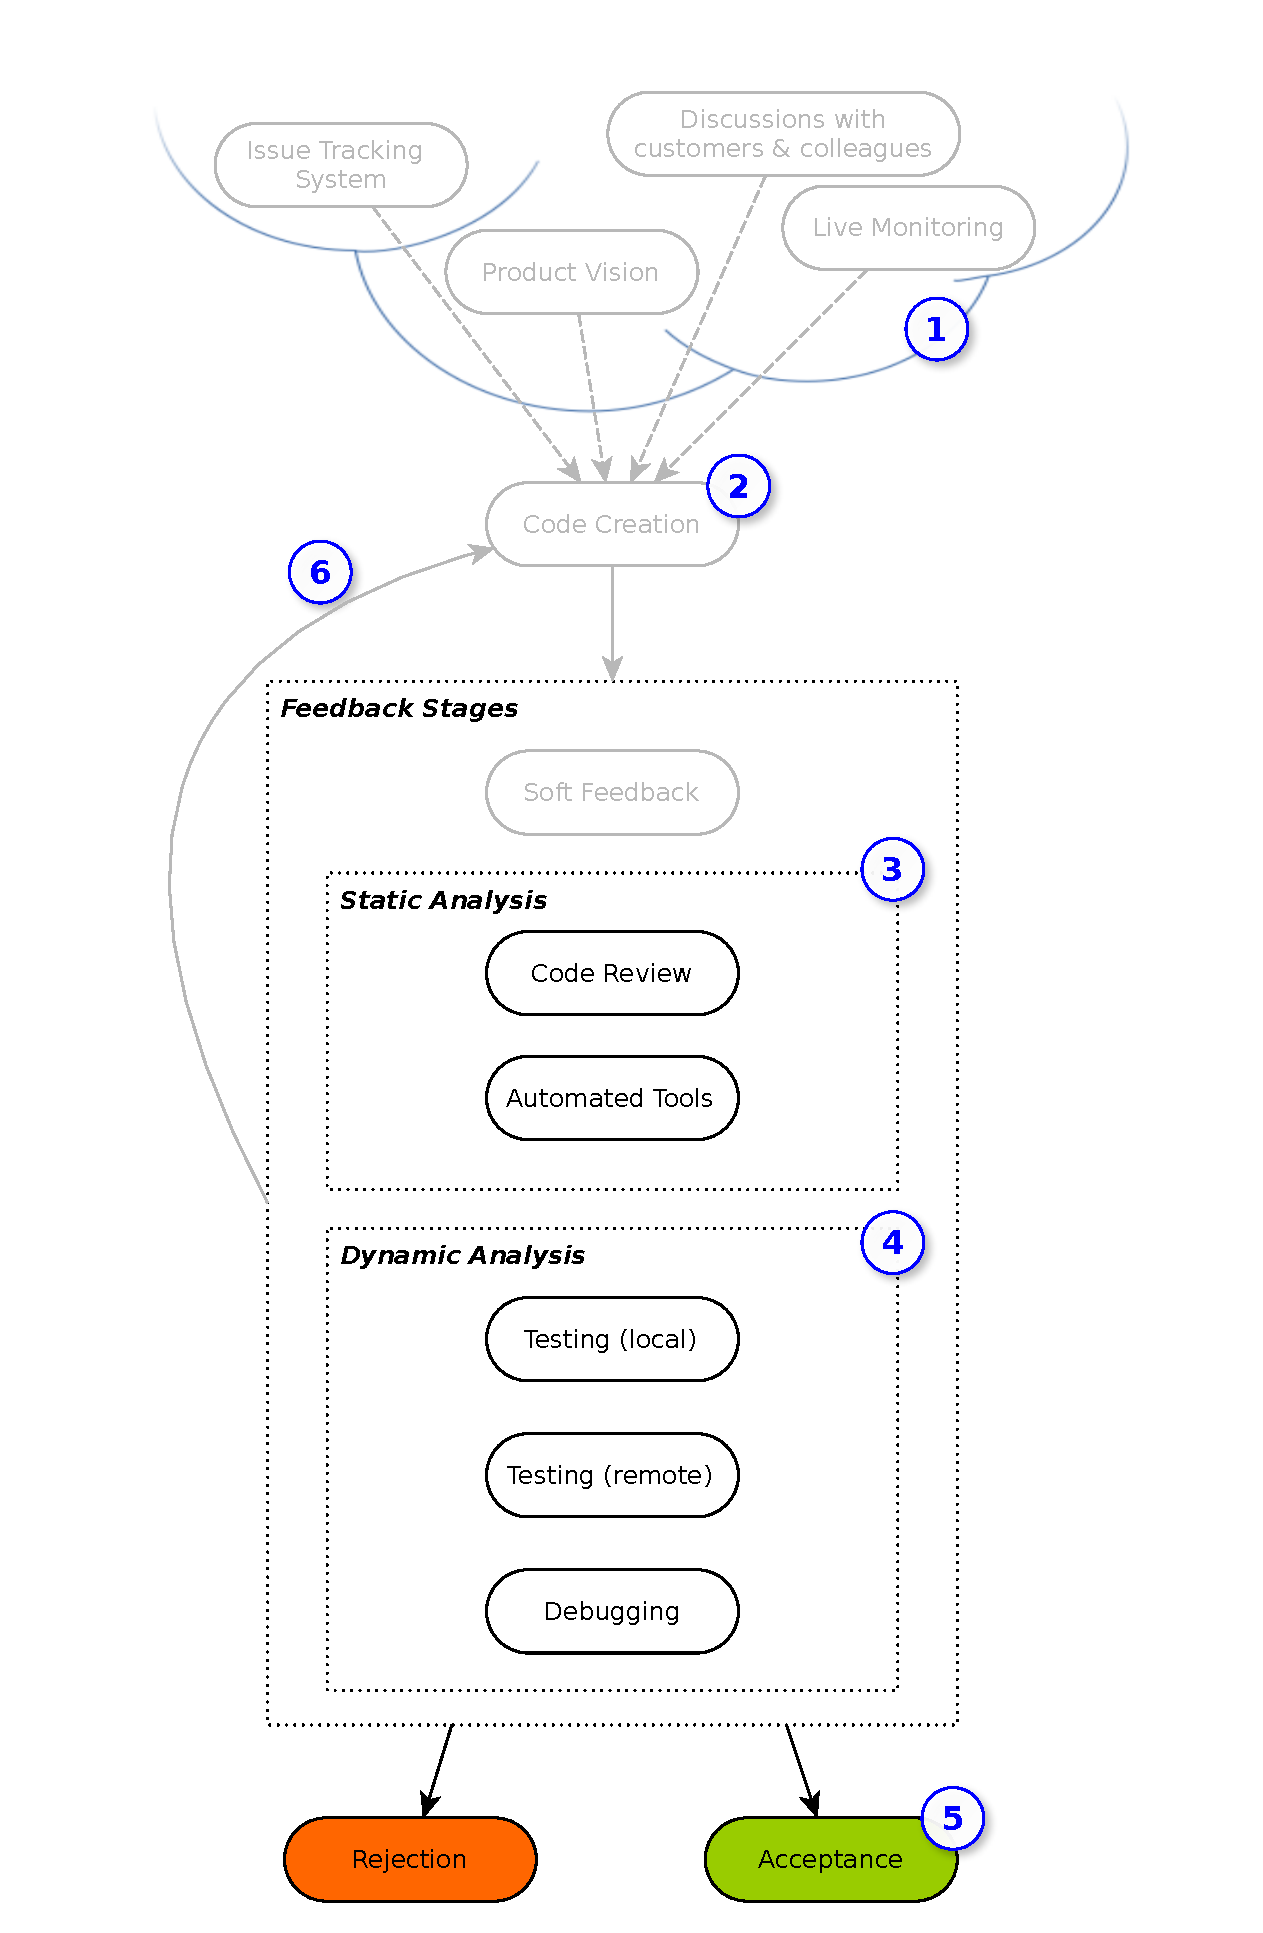
\includegraphics[width=0.65\columnwidth]{development_model_without_papers}
	\caption{The stages of the FDD model and their relationship to other
          Software Engineering concepts.}
	\label{fig:devmodel}
\end{figure}

We also have lists:

\begin{enumerate}
  \item Static Analysis~\circled{3} examines program artifacts or
    their source code without executing them~\cite{wichmann1995industrial}, while
 \item Dynamic Analysis~\circled{4} relies on information gathered from their
   execution~\cite{cornelissen2009systematic}.
\end{enumerate}

Or boxes:

\begin{framed}
This thesis is concerned with the empirical assessment of the state of the art of how developers
drive software development with the help of feedback loops.
\end{framed}

Or code:
\begin{lstlisting}[caption={\textsc{TrinityCore}},label={lst:e1}]
 x += other.x;
 y += other.y;
 z += other.y;
\end{lstlisting}


I hope this helps you get started!
Moritz

\include{asats/paper}
%
% IEEE Transactions on Microwave Theory and Techniques example
% Tibault Reveyrand - http://www.microwave.fr
%
% http://www.microwave.fr/LaTeX.html
% ---------------------------------------



% ================================================
% Please HIGHLIGHT the new inputs such like this :
% Text :
%  \hl{comment}
% Aligned Eq. 
% \begin{shaded}
% \end{shaded}
% ================================================



\documentclass[journal]{IEEEtran}

% \documentclass[12pt, letterpaper,
% twoside]{article}

% \usepackage{emoji}
\usepackage[graphicx]{realboxes}
%\usepackage[retainorgcmds]{IEEEtrantools}
%\usepackage{bibentry}  
\usepackage{xcolor,soul,framed} %,caption
\usepackage{cite}
\usepackage{multirow}
\usepackage{fontawesome}
\colorlet{shadecolor}{yellow}
% \usepackage{color,soul}
% \usepackage[pdftex]{graphicx}
% \graphicspath{{../pdf/}{../jpeg/}}
\DeclareGraphicsExtensions{.pdf,.jpeg,.png}
\usepackage{caption}
\usepackage{subcaption}
\usepackage[cmex10]{amsmath}
\usepackage[colorinlistoftodos]{todonotes}
\usepackage{hyperref} % For clickable ORCID link
\usepackage{academicons} % For ORCID icon
\usepackage{xcolor} % For colors
\newcommand{\orcidicon}{
    
\begin{tikzpicture}
    \draw[white, fill=white] (0,0) rectangle (1ex,1ex);
    \fill[green!60!black] (0, 0) rectangle (1ex, 1ex);
    \draw[white] (0.5ex, 0.5ex) circle (0.4ex);
    \draw[white, line width=0.07ex] (0.5ex, 0.5ex) -- ++(60:0.3ex);
    \draw[white, line width=0.07ex] (0.5ex, 0.5ex) -- ++(0:0.3ex);
    \draw[white, line width=0.07ex] (0.5ex, 0.5ex) -- ++(-60:0.3ex);
    \end{tikzpicture}
}
%Mathabx do not work on ScribTex => Removed
%\usepackage{mathabx}
% \usepackage{algorithm}
% \usepackage{algpseudocode}
\usepackage{comment}
% \let\hl[1]\includecomment{#1}
\usepackage{enumerate}% http://ctan.org/pkg/enumerate
% \newcommand{\hlcyan}[1]{{\sethlcolor{cyan}\hl{#1}}}
\newcommand\textblue[1]{\textcolor{blue}{#1}}
\newcommand\textred[1]{\textcolor{red}{#1}}
\definecolor{orcidgreen}{HTML}{A6CE39}

% \newcommand\myworries[1]{\textcolor{red}{#1}}
\newcommand{\orcid}[1]{\href{https://orcid.org/#1}{\textcolor{orcidgreen}{\aiOrcid}}}

\newcommand\quickthings[1]{\textblue{\\\faQuestion #1}}
\newcommand\maybelater[1]{\textred{\\\faClockO#1}}
% \newcommand\quickthings[1]{\textblue{\\\faQuestion #1}}
\newcommand\peter[1]{\textcolor{red}{\faComment #1}}
\newcommand\abs[1]{\\\hl{#1}}



%Comment to keep todo parts, Uncomment to remove TODO parts!
\renewcommand\quickthings[1]{}
% \renewcommand\absolutelynecessary[1]{}
\renewcommand\peter[1]{}
\renewcommand\maybelater[1]{}
\renewcommand\abs[1]{}
\renewcommand\hl[1]{#1}

\usepackage[linesnumbered,ruled,vlined]{algorithm2e}



% % \usepackage
% \usepackage[ruled,vlined]{algorithm2e}
% \DeclareMathOperator{\ind}{ind}
% \DeclareMathOperator{\val}{val}
% \DeclareMathOperator{\ptr}{ptr}
% \DeclareMathOperator{\row}{row}
% \usepackage{algpseudocode}
\hyphenation{op-tical net-works semi-conduc-tor}

%\bstctlcite{IEEE:BSTcontrol}


%=== TITLE & AUTHORS ====================================================================
\begin{document}
\bstctlcite{IEEEexample:BSTcontrol}
    % \title{Adversarial attacks on federarted learning for medical image analysis}
    \title{ A Comparative Study of Federated Learning Methods for COVID-19 Detection  }
 % \author{Michael~Shell,~\IEEEmembership{Member,~IEEE,}
 %        John~Doe,~\IEEEmembership{Fellow,~OSA,}
 %        and~Jane~Doe,~\IEEEmembership{Life~Fellow,~IEEE}
  
  % \author{Erfan~Darzi\href{https://orcid.org/0000-0002-6003-0119}{\includegraphics[height=1.7ex]{orcid}} ,~\IEEEmembership{Member,~IEEE},
  % Nanna~M.~Sijtsema\href{https://orcid.org/0000-0001-6644-274X}{\includegraphics[height=1.7ex]{orcid}}, and~P.M.A~van~Ooijen\href{https://orcid.org/0000-0002-8995-1210}{\includegraphics[height=1.7ex]{orcid}},~\IEEEmembership{Senior Member,~IEEE}
 

    %   and~Zoya~Popovi\'c,~\IEEEmembership{Fellow,~IEEE}% <-this % stops a space
% \\\textit{$^{1}$Machine learning lab, Data Science Center in Health (DASH) \\University of Groningen, Hanzeplein 1, Groningen, The Netherlands}
% \\ e.darzidehkalani@rug.nl
%   \thanks{ The work of Erfan Darzi was supported by KWF Kankerbestrijding and the Netherlands Organisation for Scientific Research (NWO)  Domain AES, as part of their joint strategic research programme: Technology for Oncology IL. The collaboration project is co-funded by the PPP allowance made available by Health Holland, Top Sector Life Sciences \& Health, to stimulate public-private partnerships. (\textit{Corresponding author: Erfan Darizdehkalani})\\
%   Erfan Darizdehkalani, Nanna M. Sijtsema, and P.M.A van Ooijen are with the Machine learning lab, Data Science Center in Health (DASH)
% University of Groningen, Hanzeplein 1, Groningen, The Netherlands.  (e-mail: e.darzidehkalani@rug.nl, n.m.sijtsema@umcg.nl, p.m.a.van.ooijen@umcg.nl)
  
% }
  % \thanks{Erfan Darzidehkalani is with UMCG (e-mail: e.darzidehkalani@umcg.nl).}% <-this % stops a space

% The paper headers
% \markboth{IEEE TRANSACTIONS ON MICROWAVE THEORY AND TECHNIQUES, VOL.~60, NO.~12, DECEMBER~2012
% }{Roberg \MakeLowercase{\textit{et al.}}: Cross modality image transformation using cyclic residual
% architecture and evolutionary algorithm}
% ===================================================================
\maketitle
% === ABSTRACT ====================================================================
% =================================================================================
\begin{abstract}

Deep learning has proven to be highly effective in diagnosing COVID-19; however, its efficacy is contingent upon the availability of extensive data for model training. The data sharing among hospitals, which is crucial for training robust models, is often restricted by privacy regulations. Federated learning (FL) emerges as a solution by enabling model training across multiple hospitals while preserving data privacy. However, the deployment of FL can be resource-intensive, necessitating efficient utilization of computational and network resources. In this study, we evaluate the performance and resource efficiency of five FL algorithms in the context of COVID-19 detection using Convolutional Neural Networks (CNNs) in a decentralized setting. The evaluation involves varying the number of participating entities, the number of federated rounds, and the selection algorithms. Our findings indicate that the Cyclic Weight Transfer algorithm exhibits superior performance, particularly when the number of participating hospitals is limited. These insights hold practical implications for the deployment of FL algorithms in COVID-19 detection and broader medical image analysis.
\end{abstract}
% \section{Background and Related works}

 % $\Delta W_n^t$
 
Federated learning has demonstrated efficacy in an array of imaging modalities, including Magnetic Resonance Imaging (MRI) \cite{sheller2020federated}\cite{silva2019federated}, X-ray \cite{balachandar2020accounting}, retinal imaging \cite{balachandar2020accounting}, as well as in applications such as brain tumor segmentation \cite{bakas2017advancing}\cite{lee2018privacy}, diagnosis \cite{pan2019improving}, and treatment selection \cite{lee2018privacy}. In particular, Federated Learning (FL) has proven to be a valuable tool for supporting physicians in their decision-making process regarding the treatment of COVID-19 patients. A landmark study that involved 20 institutions across five continents found that FL played a significant role in shaping patient treatment plans\cite{flores2021federated}. The study employed chest radiography images in conjunction with clinical information to determine the appropriate level of care and oxygen requirements for patients afflicted with COVID-19. It was observed that FL improved the performance of the predictive model, especially for institutions with smaller datasets, compared to using only local data for model training. Additionally, it was found that healthcare facilities with smaller datasets often had underrepresented categories due to a low number of patients in certain classes. The implementation of FL led to a notable improvement in predictions for these underrepresented patient categories.

\begin{figure*}[t!]
\centering
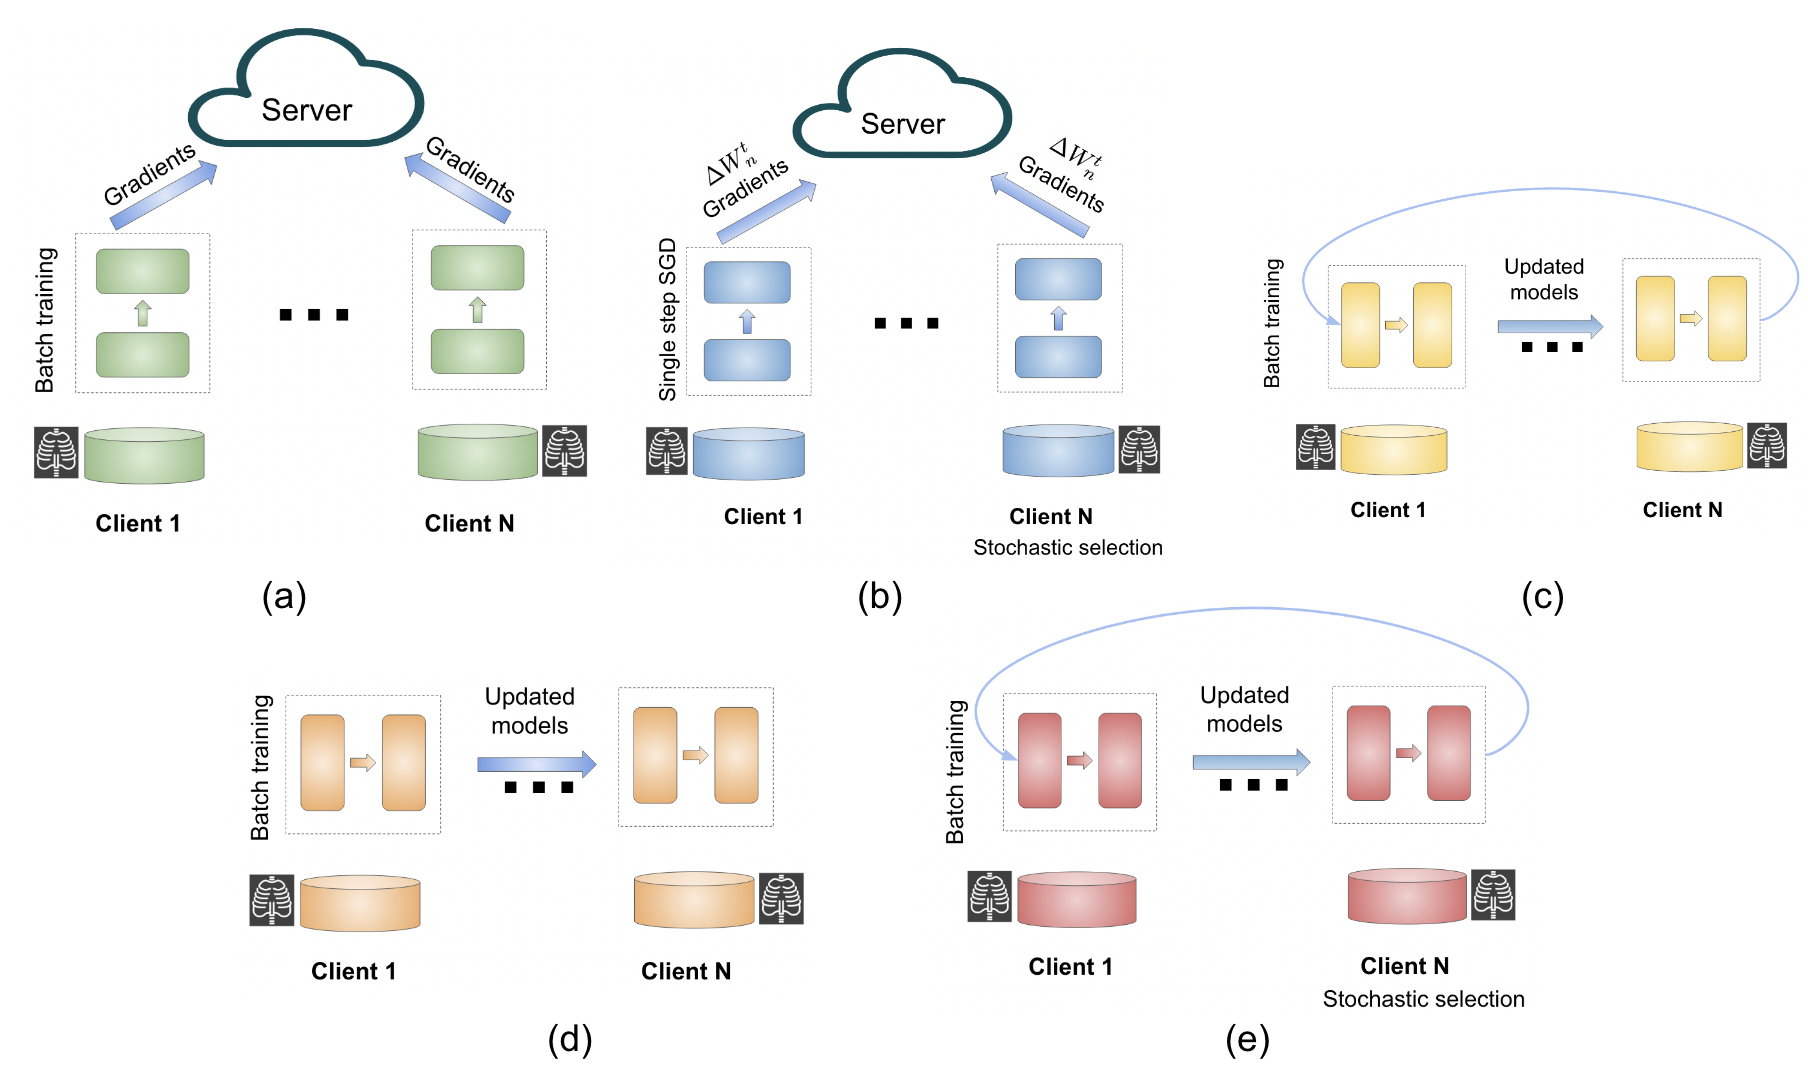
\includegraphics[width=1\textwidth]{FLmodels.png}
\caption{Illustration of FL models and algorithms: (a) Federated averaging, where clients train on a local batch of data. (b) FedSGD, in which a subset of clients is selected, and each performs a single step of SGD before sending model updates to the server. (c) Cyclic Weight Transfer (CWT), where clients train locally and pass the model to the next client, repeating the cycle. (d) Single Weight Transfer (SWT), where the model passes through each client only once. (e) Stochastic Weight Transfer (STWT), in which the model is sequentially passed through clients, with participating clients in each round being sampled randomly.}
\label{fig:flalgorithms}
\end{figure*}


Recent research has focused on the classification of scan images to distinguish between COVID-19 patients and healthy individuals, as well as identifying lesion areas. The primary application of AI in managing COVID-19 patients has been the interpretation of radiology images, especially chest CT scans.  The detection of lung alterations through these scans plays an important role in optimizing patient management and guiding treatment decisions\cite{yan2020interpretable}\cite{hu2020challenges}\cite{burian2020intensive}.  Several studies have also explored 3D Convolutional neural networks \cite{wang2020weakly} and COVID-19 detection with a limited number of training samples.

While the majority of these studies report favorable accuracy, they often presume a centralized environment wherein a single data center has access to all data. However, a few studies have successfully applied distributed learning for COVID-19 detection, employing global aggregation models such as model averaging in federated learning settings\cite{ho2022fedsgdcovid}\cite{zhang2021dynamic}, or within a blockchain framework \cite{kumar2021blockchain}. These studies have pointed to certain limitations of existing algorithms, such as high communication overhead \cite{remedios2020federated}, as well as convergence issues or catastrophic forgetting when the number of participating hospitals increases \cite{sheller2020federated} \cite{chang2018distributed}.


To our knowledge, no study has been performed that compared multiple FL algorithms under standard conditions to evaluate their applicability. Therefore, comparing multiple FL algorithms under standard conditions could be informative in evaluating their applicability in practice.

To evaluate the existing methods from multiple perspectives, we have implemented the most popular models and compared them in terms of performance, communication overhead, and computation burden.

% 
\section{Algorithms}
% \label{sec:algorithms}
\textbf{Centralized Data Sharing} In Centralized Data Sharing (CDS), data is stored in a central location and is accessible to all clients. This stands in contrast to federated and decentralized data sharing methods, where data is stored across multiple locations and accessed by either a single user or a limited number of users. CDS serves as a baseline for comparing other algorithms.
\textbf{Federated Averaging} Federated Averaging involves an iterative learning procedure comprising local and global steps. In this process, each data owner trains a model received from a global server on its local dataset through local iterations \cite{mcmahan2017communication}. Subsequently, the global server aggregates the updated local models to update the global model. This global model is then distributed to clients for the subsequent round. The optimization problem for Federated Averaging can be expressed as:
\begin{equation}
w^{t+1} = \sum\limits_{i=1}^{N}{p_{i} w_{i}^{t}} , w_{i}^{t}=\arg\min\limits_{w_{i}}{\left(\mathcal{L}(\mathcal{D}_{i};w^{t})\right)}
\end{equation}
where $N$ is the number of data owners, $\mathcal{L}(\mathcal{D}_{i};w^{t})$ is a loss function indicating global model parameters  $w^{t}$ of local datasets, and $p_{i}$ is the probability of selecting client $i$. 
Local optimization can be formulated as $w_{i}^{t+1} \leftarrow w^{t}-\eta\cdot \nabla \mathcal{L}(w^{t};\mathcal{D}_{i})$, where 
 $\eta$ is the learning rate. The global model can be updated based on the local models $w_{i}$ and is shared for aggregation: 
\begin{equation}
w^{t+1} = \sum\limits_{i=1}^{N}{p_{i} w_{i}^{t+1}}
\end{equation}

\textbf{Federated Stochastic Gradient Descent} Federated Stochastic Gradient Descent, or FedSGD\cite{chai2020fedeval}, is a variant of Federated Averaging (FedAvg) that employs a large-batch synchronous approach for multi-client learning. In FedSGD, a subset of clients is chosen from the total pool, with this subset being defined by $C$. This selection is made at each global round. Subsequently, the global server dispatches the latest global model to the chosen clients. Each of these clients then undertakes local training on its dataset for a predetermined number of epochs. The global model is updated in light of the local models obtained from each client and is made available for aggregation, a process that is analogous to that in FedAvg. Nevertheless, FedSGD distinguishes itself by computing the gradient over the chosen batch of clients, hence $C < 1$. When $C = 1$, the training becomes non-stochastic, or full batch, as it involves all the clients. This makes it possible to train with large batches since the gradient is computed over the selected subset of clients.

The optimization problem for FedSGD can be expressed as follows:
\begin{equation}
w^{t+1} = w^{t} - \eta \cdot \sum\limits_{i=1}^{C}p_i \cdot \nabla \mathcal{L} (w^t;\mathcal{D}_i)
\end{equation}
where $\eta$ is the learning rate, $p_i$ is the probability of selecting client $i$ and $\mathcal{L}$ is the loss function.
The key difference between FedAvg and FedSGD lies in the use of large-batch synchronous approach in FedSGD. This approach has been shown to outperform the naive asynchronous SGD training due to the increased accuracy and efficiency, as compared to the local training approach used in FedAvg \cite{chai2020fedeval}\cite{charles2021large}. Additionally, FedSGD has been shown to be more robust to non-IID data distributions, compared to FedAvg \cite{chai2020fedeval}. 
\quickthings{This part is unclear to me.}
% \absolutelynecessary{}
\maybelater{paraphrised}

\textbf{Cyclic weight transfer} Federated learning techniques have been widely used in medical image processing tasks using a method known as cyclic weight transfer (CWT)\cite{balachandar2020accounting}. This method involves training models on individual clients for a number of iterations and then cyclically sharing the updated weights with the following client. However, the existing CWT algorithm faces a notable challenge, as it lacks the ability to effectively manage inter-client variability in training data or labels.  To ensure the practical application of CWT, it is crucial to develop a version that can handle the common variations observed in a majority of real-world medical imaging datasets\cite{darzidehkalanifederatedII}.

\textbf{Single weight transfer} Single weight transfer (SWT) is anothe FL method widely used in the medical imaging domain. In Single weight transfer, models are trained in each client with its local data, and then the updated model is transferred to the next client. The difference between this method and CWT is that here the model passes each client only once\cite{darzidehkalanifederatedI}. 

\textbf{Stochastic weight transfer}
In stochastic weight transfer (STWT), we select a subsample of clients and train them in a cyclic manner. Similar to FedSGD, a ratio defines the number of selected clients to the total number of clients in each federated round. 

Figure \ref{fig:flalgorithms} provides a visual representation of the introduced algorithms.



% سوال / مسیله چیه
% Importance: Why your research matters in the context of an industry or the world
% اهمیت موضوع
% 	کجاها کاربرد داره
% مشکلات موضوعات قبلی و اینکه مسایل دگ کار نمیکنن
% برای اینکه این مسایل کار کنن نیازی به چه چیزی بود. ک اونا کم داشتن
% چرا این روش تو داره کار میکنه
% چه سوالی رو جواب میده
% توضیح اینکه چجوری کار میکنه
% تعریف و تمجید از کار کردنش

% \maybelater{chanta akse tamiz ba coreldraw bekesh}

% Their
% We are comparing various implementations of FL and comparing their performance level. The performance is done by metrics.
% 2. Although FL has been introduced to tackle the problem of privacy, its distributed nature requires too much commuincation between clients. Knowsing can determine its deployability and scailibitlty. Hence the question is how to these model compare it terms of communication between clients.
% 3. Computation time. Each FL model is investigated based on the required time for computation.
% 4. Effect of rounds: Number of Federated rounds 


% \quickthings{Maybe you can add a benchmarking section similar to "A Performance Evaluation of FL Algorithms"}
% \maybelater{Some ideas are herer https://arxiv.org/pdf/1709.05929.pdf
% }



% 

 
\section{Experiment}
\textbf{Dataset} Our experiments used two publicly available data sources, the Tongji hospital dataset\cite{yang2020covid} and Brazil's SARS-CoV-2 dataset\cite{soares2020sars} Tongji dataset consists of 349 chest CT-scans of COVID-19 positive and 397 scans of healthy subjects, all low-resolution CT modalities. Brazil's SARS-CoV-2 dataset consists of 2482 samples, 1252 scans of COVID-19-infected patients, and 1230 healthy subjects collected from multiple hospitals in Sao Paulo, Brazil. The datasets are approved by the corresponding ethical committees of each hospital, Public Hospital of Sao Paulo (HSPM), and Tongji Hospital in Wuhan, China. Train and test sets were obtained randomly from the aggregated datasets. Table \ref{table_datadist}, shows data distribution.


\begin{table}[h!]
\centering
\setlength{\tabcolsep}{6pt}
\renewcommand\arraystretch{1.22}
\caption{ \small Data distribution}
\begin{tabular}{| *{5}{c|} }
\hline
Class  & Dataset & Samples & Train & Test
\\   \hline  
\multirow{2}{3em}{COVID}     &Brazil&1252&\multirow{2}{2em}{1451}  &\multirow{2}{2em}{150}  \\
&Tongji&349&&  \\
\hline
\multirow{2}{6em}{Non-COVID}     &Brazil&1230&\multirow{2}{2em}{1477}  &\multirow{2}{2em}{150}  \\
&Tongji&397&&  \\
\hline
\end{tabular}
\label{table_datadist} 
\end{table}


\textbf{Preprocessing}
Images were selected as 2D slices in greyscale. Preprocessing included randomly cropping between 0.5 to full size, random horizontal flipping, and intensity normalization. CT-slices were all resized to 224$\times$224 pixels with interpolation. Figure \ref{fig:samplesCTs} shows samples of processed images.
% \quickthings{This looks like you have a bias in your dataset. You should select the normals and abnormals at comparable level in the thorax. All covid are now lower in the body then the non-covid ones.}
% \maybelater{I have changed the picture, hope it's okay now}
\begin{figure}[h!]
 \centering
 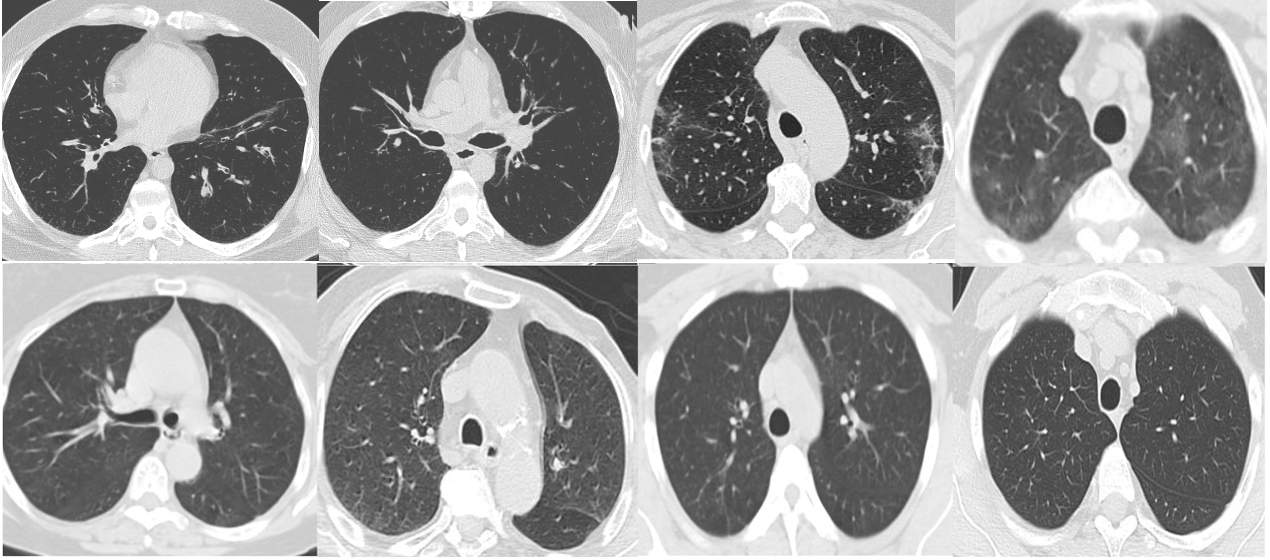
\includegraphics[width=0.45\textwidth]{covidexamples3.png}
 \caption{Sample CT slices of COVID-19 images (top row) and Non-COVID images (bottom row)}
 \label{fig:samplesCTs}
\end{figure}


% normalize = transforms.Normalize(mean=[0,0,0], std=[1,1,1])
% train_transformer = transforms.Compose([
%     transforms.Resize(256),
%     transforms.RandomResizedCrop(224, scale=(0.5, 1.0)),
%     transforms.RandomHorizontalFlip(),
%     transforms.ToTensor(),
%     normalize
% ])

\textbf{Training}
ResNet-18 is used as the backbone deep learning model. ResNet-18 comprises one initial block cascaded to four middle blocks. The initial block is made of convolutional,  batch normalization, ReLU, and pooling layers. Middle blocks have the same layers, connected with straight and skip connections. The model is pre-trained on ImageNet dataset \cite{he2016deep} with a CrossEntropy loss function and learning rate of $0.05$. 
Each federated round consisted of 20 internal epochs for each client and batches of 16 samples in each iteration. For models which use minibatch training, like STWT and FedSGD, a subset of clients is randomly selected. Similar to training, test data was split into mini-batches, and the results were averaged across batches. We performed training with various participating clients and federated rounds to evaluate their effect on final performance. Models were also trained in a centralized, non-federated setting to build a comparison baseline. Figure \ref{fig:distributionsite} shows the data distribution among clients.

\begin{figure}[h!]
 \centering
 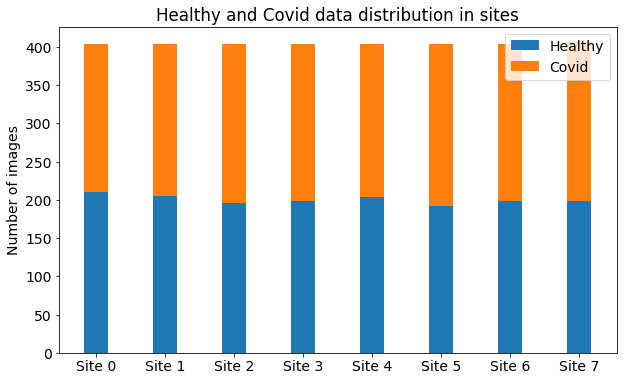
\includegraphics[width=0.7\textwidth]{output.png}
 \caption{Data distribution of each client in the simulated federated setting}
 \label{fig:distributionsite}
\end{figure}
% \abs{Healthy COVID data distirbution per site}

\textbf{Evaluation} 
Standard classification metrics, accuracy, recall, precision, and F1 score, were used as our evaluation criteria. We also evaluated the level of communication, the amount of transferred data in each algorithm, and the computational complexity of the models. 
\label{sec:experiment}


% \section{Results}


% In order to evaluate and compare federated learnign models 
% Specificity  and  sensitivity  are  the  abilities  of  a  model  that how correctly the model identifies a subject with disease and without a disease. 
% In our case, it is critical to detect a COVID-19 patient as missing a COVID-19 patient can have disastrous consequences.   

% A medical diagnosis based system needs to have high sensitiv- ity and recall. 
Here, the result for the setting with 10 participating clients and a maximum of 10 rounds is presented. The results are average performance among clients for all the federated rounds. Table \ref{best_performance} shows the results.
% \quickthings{Why comparison of FedAVG and CWT?}\maybelater{I removed the sentence}
% The average score in each state could be a way to reach them—the average scores in F1, FedSGD, CWT, and SWT. 
% The FedSGD models have been used are
% The results for CDS are also included as a benchmark ground truth.

% \quickthings{Put CDS at the top, keep same order as in the materials and methods. Consistency!}
% \maybelater{Fixed!}

\begin{table}[h!]
\centering
\setlength{\tabcolsep}{5.5pt}
\renewcommand\arraystretch{1.12}
\caption{ \small Comparison of FL algorithms on classification of COVID-19 data for 10 clients, averaged performance in all the 10 rounds.}
\begin{tabular}{| *{5}{c|} }
\hline
Method & Accuracy & Recall & Precision & F1 score
\\
  \hline
  

CDS
 &87.75\%&89.57\% &87.93\% & 87.19\%  
\\   \hline  
FedAVG
 & 66.72\% &70.02\% &43.80\% & 51.7\%\\ 
 \hline  
FedSGD
 &65.17\% &68.24\%&43.86\%& 47.75\%  
 
 \\
 \hline  
CWT
 &87.75\%&89.00\%& 88.67\%&87.52\%\\
 
   \hline
 

SWT
 & 64.60\% &74.33\% & 65.55\% &59.66\% \\
    
\hline 
STWT
 & 84.21\% &84.09\%&83.33\% & 81.71\%  \\



\hline
\end{tabular}
\label{best_performance} 
\end{table}


\textbf{Assesing the impact of training rounds} To evaluate the effect of number of rounds, models with 3, 5, 10 and 15 rounds were tested. The test results are shown for both centralized and FL  algorithms. Table \ref{number_of_rounds} shows the results of our experiment. The increasing number of rounds correlates with higher accuracy of the global model.
% \quickthings{Same with table III, put at the top.}

% \maybelater{done}

% \begin{table}[h!]
% \centering
% \setlength{\tabcolsep}{5.5pt}
% \renewcommand\arraystretch{1.12}
% \caption{ \small Effect number of rounds on models' accuracy}
% \begin{tabular}{| *{5}{c|} }
% \hline
% Method & 3 rounds & 5 rounds & 10 rounds & 15 rounds 
% \\   \hline  
% FedAVG
%  & 66.28\% &77.24\% & 86.63\% & 94.03\%\\

%  \hline
%  FedSGD
%  &  53.77\% & 70.55\% &90.04\% & 92.75\%\\
% \hline  
% % SWT
% %  &  85.34\% & 97.24\% &93.63\% & 98.74\%\\
% % \hline  
% CWT
%  &  96.02\% & \textbf{98.44\%} &\textbf{99.29\%} & 99.86\%\\

% % \hline  
% % CDS
% %  to be completed!


% \hline  
% STWT
%  &  \textbf{96.59\%} & 97.72\% &99.57\% & \textbf{100.00\%}\\

 
%  \hline
% CDS
%  &92.03\% &88.34\% & 98.01\% & 100.00\% \\
%  \hline
% \end{tabular}
% \label{number_of_rounds} 
% \end{table}


\begin{table}[h!]
\centering
\setlength{\tabcolsep}{3.5pt}
\renewcommand\arraystretch{1.12}
\caption{ \small Effect number of rounds on accuracy of FL algorithms for 10 clients, 20 internal epochs.}
\begin{tabular}{| *{5}{c|} }

% \begin{tabular}{| {c|}{c|}{c|}{c|}{c|}{c|}{c|}{c|}{c|} |}
\hline
% Method & \multicolumn{2}{c}{3 rounds} & \multicolumn{2}{c}{5 rounds} &\multicolumn{2}{c}{10 rounds} &\multicolumn{2}{c}{15 rounds} 

Method & 3 rounds & 5 rounds & 10 rounds & 15 rounds
%  & M &SD & M &SD& M &SD& M &SD 
\\
 \hline
CDS
 &85.06\% &81.56\% & 91.06\% & 91.04\% 
\\
\hline
FedAVG
 & 56.05\%  &63.78\%&69.64\%&70.73\% \\

 \hline
 FedSGD
 &  50.88\% & 55.9\% &75.59\% & 76.94\%\\
% \hline  
% SWT
%  &  85.34\% & 97.24\% &93.63\% & 98.74\%\\
\hline  
CWT
 &  80.77\% & \textbf{89.78\%} &\textbf{91.27\%}& \textbf{93.56\%}\\

% \hline  
% CDS
%  to be comp,';leted!


\hline  
STWT
 &  \textbf{90.73\%} & 83.97\% &89.44\% & 93.01\%\\

 
  \hline

\end{tabular}
\label{number_of_rounds} 
\end{table}
\quickthings{Shouldn't this column have the same results as table II for accuracy?}

\peter{Table III and Table II do not represent the same thing. Table II is average performance in all 10 rounds, is to give an overall impression of accuracy, and table III is the final result in the end of the 5th, 10th , 15th rounds.  Added  to the table caption.
}
% \maybelater{The results are for max, maybe you want to add average results later?}
% \maybelater{Having the same thing (acc) for other metrics such as F1, prevciison recall etc}

\textbf{Assessing the influence of client participation}
To evaluate the number of clients on the FL network, we examined scenarios with 3,5, and 8 participating clients. We trained each of the clients in 20 internal epochs. The number of Federated rounds for all the algorithms (except SWT) was 10.
The average test results are shown in the Figure \ref{fig:data distribution}. \quickthings{Why not a column for 10 clients here?}
\maybelater{ 10 clients are shown in table three , third column. Added 10 clients here as well}

% \begin{table}[h!]
% \centering
% \setlength{\tabcolsep}{7pt}
% \renewcommand\arraystretch{1.22}
% \caption{ \small Effect number of clients on accuracy of FL algorithms, 10 rounds, 20 internal epochs.}
% \begin{tabular}{| *{9}{c|} }
% \hline
% Method & 3 clients & 5 clients & 8 clients 
% \\   \hline  
% FedAVG
%  & 79.52\% &70.73\% & 63.98\% \\

% \hline  
% FedSGD
%  & 78.02\% &75.59\% &69.76\%  \\
% \hline  
% CWT
%  &  89.90\% & \textbf{91.27\%} &\textbf{88.98\%} \\
%  \hline
% STWT
%  &  \textbf{90.93\%} & 89.44\% &84.57\% \\
%  \hline  
% SWT
%  & 55.80\% &69.19\% & 68.81\%\\




% \hline  
% CDS
%  to be completed!

% \hline  

% \end{tabular}
% \label{effect_num_clients} 
% \end{table}


\begin{figure}[h!]
 \centering
 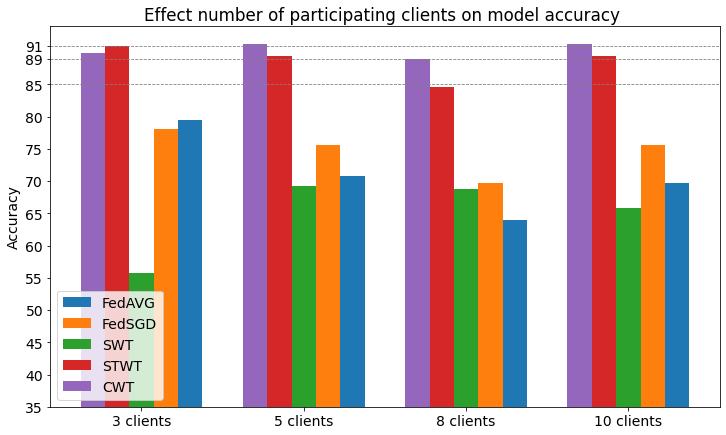
\includegraphics[width=0.7\textwidth]{download.png}
 \caption{Accuracy of FL algorithms with differrent number of clients. }
 \label{fig:data distribution}
\end{figure}


% \maybelater{Maybe taking MAX is better instead of latest epoch?}

 
\begin{figure}[h!]
 \centering
 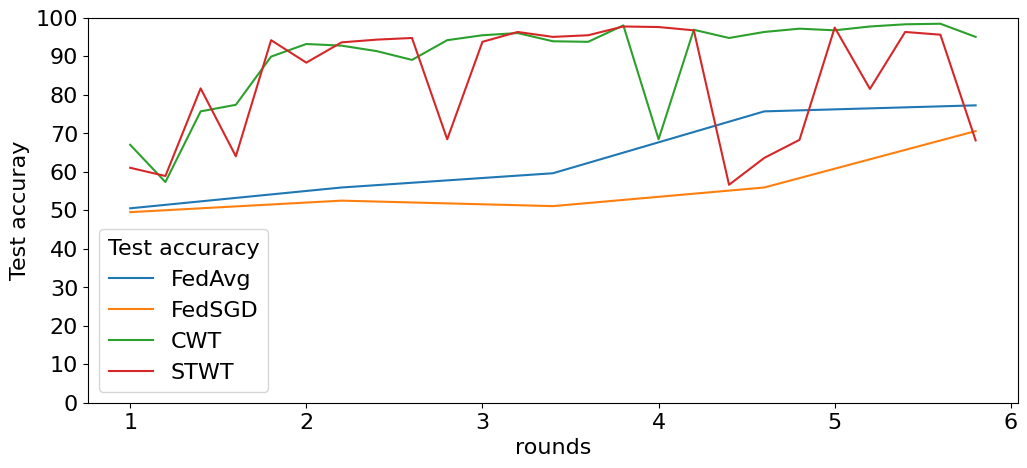
\includegraphics[width=0.7\textwidth]{cyclic.png}
 \caption{Test accuracy as a function of passing rounds}
 \label{seq-vs-noseq}
\end{figure}
% \maybelater{Best accuracy vs Average accuracy for showing that SWTW works bad in average but well in best accuracy}
% \abs{Adding a graph showing arrows for gradient updates}
% \maybelater{Maybe adding 10 clients?}
% \maybelater{8 ta client, 4 FL rounds
% 20 each client for CWT plot . and also 8 ta client, 4 FL round 20 each client for FedSGD and FedAVG}
% \subsection{Other graphs}

\begin{table}[h!]
\label{computation time}
\centering
\setlength{\tabcolsep}{7pt}
\renewcommand\arraystretch{1.22}
\caption{ \small Computation time (seconds) for FL algorithms for standardized setting}
\begin{tabular}{| *{9}{c|} }
\hline
Method & 3 clients & 5 clients & 8 clients  & 10 clients
\\   \hline  
FedAVG
 & 8934 sec&8975 sec  & 9002 sec & 9030 sec\\

\hline  
FedSGD
 & 8810 sec &8853 sec& 9013 sec & 9052 sec \\
\hline  
CWT
 &  5119 sec& 5450 sec&5383 sec & 5556 sec\\
 \hline
STWT &
2805 sec&  5243 sec& 6101 sec & 6129 sec\\
 \hline  
SWT
 & \textbf{543 sec} &\textbf{547 sec} & \textbf{589 sec } & \textbf{618 sec}\\



% \hline  
% CDS
%  to be completed!

\hline  

\end{tabular}
\label{computation_time} 
\end{table}


Communication can also be a bottleneck in this setting. In methods like federated averaging, the lower bounds for total communicated data are proportional to $\sim$
${2NT}$
where the total rounds are represented by T and the count of involved clients is denoted by N. In CWT, this lower bound is  $\sim$ ${NT}$. In our setting, we use a ResNet 101 model. We calculated the overall transferred data for the different number of rounds. As expected, the experiments show that when clients are selected randomly, the communication time tends to be shorter compared to scenarios involving participation from all clients. Moreover, our analysis of computational costs indicates that models that do not rely on sequential processing generally demand higher computational resources compared to their sequential counterparts. The detailed results for computational and communication evaluations can be found in Table \ref{computation_time} and Table \ref{transferredData}, respectively.
\quickthings{Again, why only this comparison is relevant enough to put into the text?}
\maybelater{Here fedavg, and fedsgd are the same family, (non sequential), and CWT are the other family (sequential)., Changed the phrasing from CWT/FedAVG to seq/non-seq, hope it's okay this time.}

\begin{table}[h!]
\centering
\label{Transferred data}
\setlength{\tabcolsep}{5.5pt}
\renewcommand\arraystretch{1.12}
\caption{ \small Comparison of total transferred data in a normalized setting (GB)}
\begin{tabular}{| *{5}{c|} }
\hline
Method & 3 rounds & 5 rounds & 10 rounds & 15 rounds 
\\   \hline  
FedAVG
 & 1.371 &2.286 & 4.571 & 6.857\\

 \hline
 FedSGD
 &  0.823 & 1.371 &2.743 & 4.114\\
\hline  
% SWT
%  &  85.34\% & 97.24\% &93.63\% & 98.74\%\\
% \hline  
CWT
 &  0.686 & 1.143 &2.286 & 3.428\\

% \hline  
% CDS
%  to be completed!


\hline  
STWT &
  0.411 & 0.686 &1.371 & 2.057\\

 

 \hline
\end{tabular}
\label{transferredData} 
\end{table}





% \maybelater{Momkene computational complexity ro beshe ba order nevesht? peida kon settingesh ro}
% \maybelater{Graphs showing results}
% \maybelater{Comparison of FL models}
% \maybelater{Loss/round}
% \abs{definition of precision and recall}


\label{sec:results}



% % \newpage

% 
\section{Discussion}
\label{sec:discussion}

% Local training had near random accuracy, but in all the experiments, the performance results were improved. 
% Considering low number of samples for individual clients, a training process limited to few clients results in near random classification accuracy. 
% Local models can have low performance due to limited datasets.
% Also,, ImageNet pre-training had a speed-up effect on our model performance.

% \textbf{Fundamental groups of FL}

% \textbf{how many groups}
% \textbf{how can we group them, name different ways}
% \textbf{effect number of data}


% Paragraph 1: This paragraph provides a “big picture” perspective for readers to remind them of the importance of your study.

% \textbf{overall results}
% 
Our results show that FL has comparable performance to centralized data sharing, with the advantage of keeping data private. With large volumes of data and after high number of rounds, centralized data sharing and cyclic weight transfer have the highest accuracy. 


Sequential models are susceptible to catastrophic forgetting, where a global model performs well on the latest client it has seen while having poor performance in other clients.\quickthings{cryptic sentence}\maybelater{I have paraphrised the sentence}
Conversely, in algorithms like FedAvg and FedSGD, the models are averaged asynchronously after all the clients have finished their training. So the trajectory is smoother and overall improving with more communication rounds. As shown in Figure \ref{seq-vs-noseq}, local test results can have a high variance when passing through clients sequentially, indicating the catastrophic forgetting effect.

Models like FedAvg, and FedSGD, in which all the clients have identical copies of one global model, are slower and more challenging to converge compared to sequential models like CWT and STWT. Also, FedAvG and FedSGD require more training resources due to active server participation, resulting in more computation and network consumption. Stochastic client selection is an efficient way of training. Stochastic models save significant time and resources while having similar performance to full client participation. Overall, CWT and STWT have best results in terms of model accuracy and computation times. These findings could be practical in further federated deployments in medical institutions.
% but when there are communication and computation limitations, other methods might be more practical.




% As can be seen in the results, CWT and STWT have better local results than other methods.

% So each local model is different than other models, and even in fewer rounds they retrain the model on their local data and achieve high accuracies. 

%  Unsurprisingly, CDS has higher accuracy than non-sequential methods.
 
% so in limited number of rounds, latter algorithms are preferred.



%  FedAVG needs to perform both local training and global aggregation, which requires is to have more computation, than sequential models which eliminate global aggregation and broadcasting step.   
%  Models with global server, suh as FedAVG and FedSGD, required more data transfer, because of the two way communication of each client with server.
Sequential models like CWT and STWT perform better than non-sequential models on fewer training rounds. For example,  after three rounds of training, STWT and CWT both reach 96\% accuracy, while FedAvG reaches 66\%, and FedSGD performs equally to a random classifier. As the training proceeds, FedAVG and FedSGD gradually improve with more global rounds.The concept of sequential models is similar to fine-tuning \cite{chen2020online} in centralized deep learning, so in cases where a hospital temporarily joins an FL network, or there is an urgency in training, sequential models are a better option.

More training rounds do not always lead to a better global model. Although average performance on all clients improves, more global rounds lead to worse performance for some clients. The global model can overfit some clients, leading to lower performance on others\cite{mohri2019agnostic}. Some studies suggested early stopping and fine-tuning to local dataset after global training is finished \cite{yu2020salvaging}. 
In all the algorithms, more clients resulted in slower convergence. This effect is stronger in the FedAvg algorithm. In FedAVG, the Global model must compromise between potentially disparate local minima\cite{li2019convergence}. Methods such as adaptive or stochastic selection of clients and momentum-based models help faster convergence \cite{liu2020accelerating}.
Our results suggest that stochastic client participation is close to full client participation. The average results of four trials with varying rounds, shown in Table \ref{number_of_rounds} indicate that stochastic client participation in FedSGD results in 5.23\% performance loss and 40\% less bandwidth consumption compared to FedAvg. In STWT, it results in only 1.25\% less accuracy but saves 40\% of communication and 11.3\% of computation.
% Also, SWT improves local clients' performance up to 80\% accuracy with 8 clients, and it requires extremely low bandwidth requirements.
These results are in accordance with prior studies, showing that, in theory, stochastic and full client participation have similar global minima\cite{cho2020client}. Stochastic client selection can be advantageous when there are limited resources, or in larger networks with occasionally unavailable clients.


% Models like FedSgd and STWT, select the participating clients in a stochastic manner. 
% The reason is because each client has less data, and there will be more number distant local client minima leading to unstable global model.


% Such can be a reflection of real world setting, where not all the clients are active in each round. So a fraction are selected.


% Some models have high max test accuracy while average is low indicating bias and catastrophic forgetting. Infrastructure limitations should be considered, when a central server has limited computing power it would be unable to perform FedAVG, instead no-server algorithms require to pass the model to the next client.

We did not assume any shift in clients' data. A more comprehensive analysis should consider the effect of the domain and distribution shifts on the performance of the algorithms. Also, inter-client data variability and the effect of heterogenous clients could be a future line of research.
% For deployments in longer timeframes, there might be changes in clients data distirbution , and previous results might be inapplicable Effect of domain shifts, and inter-client data variability could be a future line of research. 






\section{Conclusion}
\label{sec:conclusion}
 
FL enables extensive collaborations of hospitals to address medical imaging problems while keeping data private. Real-world implementation requires consideration of efficiency and hardware requirements in addition to model performance, especially in the healthcare field, which generally has limited infrastructure. We implemented five FL algorithms for COVID-19 detection and analyzed their efficiency and accuracy.
Our results suggest that FL algorithms have comparable performance to centralized data sharing, with the advantage of keeping data private. They also show that the sequential methods are a better option in most of the scenarios. This study can be helpful in the deployment of FL systems in COVID-19 detection and medical image analysis in general.

% demonstrate better performance for detecting COVID-19 patients and might be practical in deploying FL algorithms for covid-19 detection and medical image analysis in general.





\printbibliography







% === KEYWORDS
% ====================================================================
% =================================================================================
\begin{IEEEkeywords}
federated learning, medical image analysis, COVID-19, privacy preserving machine learning
\end{IEEEkeywords}






% For peer review papers, you can put extra information on the cover
% page as needed:
% \ifCLASSOPTIONpeerreview
% \begin{center} \bfseries EDICS Category: 3-BBND \end{center}
% \fi
%
% For peerreview papers, this IEEEtran command inserts a page break and
% creates the second title. It will be ignored for other modes.
\IEEEpeerreviewmaketitle


% ====================================================================
% ====================================================================
% ====================================================================










% \tableofcontents
% === I. INTRODUCTION =============================================================
% =================================================================================
\section{Introduction}

\IEEEPARstart{C}oronaviruses comprise a family of viruses known to cause respiratory and intestinal illnesses in both humans and animals. Among these viruses, the variants responsible for COVID-19, SARS, and MERS epidemics have gained notable attention. In cases of COVID-19, certain individuals might develop severe complications, including pneumonia, which can be detected through lung CT scans. Studies have indicated that chest imaging plays a crucial role in the diagnosis of COVID-19 in individuals exhibiting severe symptoms. In this domain, deep learning methods, especially Convolutional Neural Networks (CNNs), have proven to be highly effective in assisting radiologists in performing various image analysis tasks related to the diagnosis of COVID-19\cite{kogilavani2022covid}.

Deep learning models developed specifically for detecting COVID-19 infections have exhibited remarkable potential in identifying infected regions in CT scans and X-ray images. However, the training of these deep learning models necessitates access to ample and diverse medical datasets, which are typically collected from multiple sources. A majority of the current approaches rely on a centralized server for aggregating data from various healthcare institutions. This approach poses a challenge, as medical images often contain sensitive and confidential patient information, which is not permissible to share beyond the confines of the originating institution.

Federated learning (FL) emerges as a viable solution to this challenge by decentralizing the training process and retaining the data at its source. In a federated learning framework, distinct clients participate in the training process in a distributed manner using their local data. Specifically, each client independently trains a model utilizing its dataset and subsequently shares the model parameters with other participants. Crucially, the actual data does not leave the local premises, thereby maintaining the confidentiality of sensitive patient information. This approach facilitates collaborative learning without compromising data privacy.
% the distributed computation and develpmoent of deep learning models ensure the accumulation of knowledge and reaching the full capacity of deep learning models.

FL can differ from centralized data sharing in a number of ways. While both approaches aim to optimize their learning objective, FL algorithms have to account for the fact that communication with clients takes place over unreliable networks with very limited upload speeds. So unlike 
the centralized setting in which computation is generally a bottleneck, in FL communication might be the bottleneck. 

In this study, a framework was developed to facilitate collaboration among hospitals by employing multiple data sources for the detection of COVID-19 infections via FL. The framework's decentralized data distribution ensures privacy, as data remains stored locally\cite{darzidehkalanifederatedII}.




% There are several ways of doing federated learning since federated learning is performed in a higher level compared to conventional deep learning. There are more parameters of complexity since the model should take into consideration the general and local methods of optimization, data accumulation for all the sites, and local training models. 
% There are several parameters playing a role in the final performance of a federated learning setting.

 





% It can be spread by human-human interaction. There are several waus tp diagnose COVID-19. Transcription-polymerase chain reaction (RT-PCR) test are one of the most common ways of diagnosing COVID-19. However, there are other ways of diagnosing COVID-19 \cite{rubin2020role}
% However, due to large number of people having the symptoms and being tested for COVID-19, it might not always be feasible for radiologists to examine large number of patients during the outbreak. Scans of CT and Xray of infected patients have sorts of deformation, misalignment between certain parts, or have pixel intensities different than normal people in infected parts. Observing this misalignment in not an easy task and requires effort and focus from radiologist to correctly distringuish betweeen healthy and infected people. 
% Instead, 
% Various architectures of CNN have been tested  and shown a great performance on the imaging datasets. Models such as AlexNet \cite{krizhevsky2012imagenet}
%  ResNet \cite{he2016deep}  and MobileNet \cite{howard2017mobilenets} could classify thousands of objects belonging to hundreds of classes with the same accuracy as human.
 



% It has also been used to detect COVID-19 from imaging data. Most of the usecases were either for Xray like the researches in 
% While CT scans can help screen COVID-19 potential infected people, CT scans of other diseases could also have overlapping features with COVID ingected patients. Hence, it is tricky to distinguish COVID infected patients from other types of lung inflammation and requires radiologists level experrtise. The most literature focuses on the ways to better distirnguish COVID infected patients from other diseases, as can be seen in [8], [9], [10], [11], [12]. 

\section{Background and Related works}

 % $\Delta W_n^t$
 
Federated learning has demonstrated efficacy in an array of imaging modalities, including Magnetic Resonance Imaging (MRI) \cite{sheller2020federated}\cite{silva2019federated}, X-ray \cite{balachandar2020accounting}, retinal imaging \cite{balachandar2020accounting}, as well as in applications such as brain tumor segmentation \cite{bakas2017advancing}\cite{lee2018privacy}, diagnosis \cite{pan2019improving}, and treatment selection \cite{lee2018privacy}. In particular, Federated Learning (FL) has proven to be a valuable tool for supporting physicians in their decision-making process regarding the treatment of COVID-19 patients. A landmark study that involved 20 institutions across five continents found that FL played a significant role in shaping patient treatment plans\cite{flores2021federated}. The study employed chest radiography images in conjunction with clinical information to determine the appropriate level of care and oxygen requirements for patients afflicted with COVID-19. It was observed that FL improved the performance of the predictive model, especially for institutions with smaller datasets, compared to using only local data for model training. Additionally, it was found that healthcare facilities with smaller datasets often had underrepresented categories due to a low number of patients in certain classes. The implementation of FL led to a notable improvement in predictions for these underrepresented patient categories.

\begin{figure*}[t!]
\centering
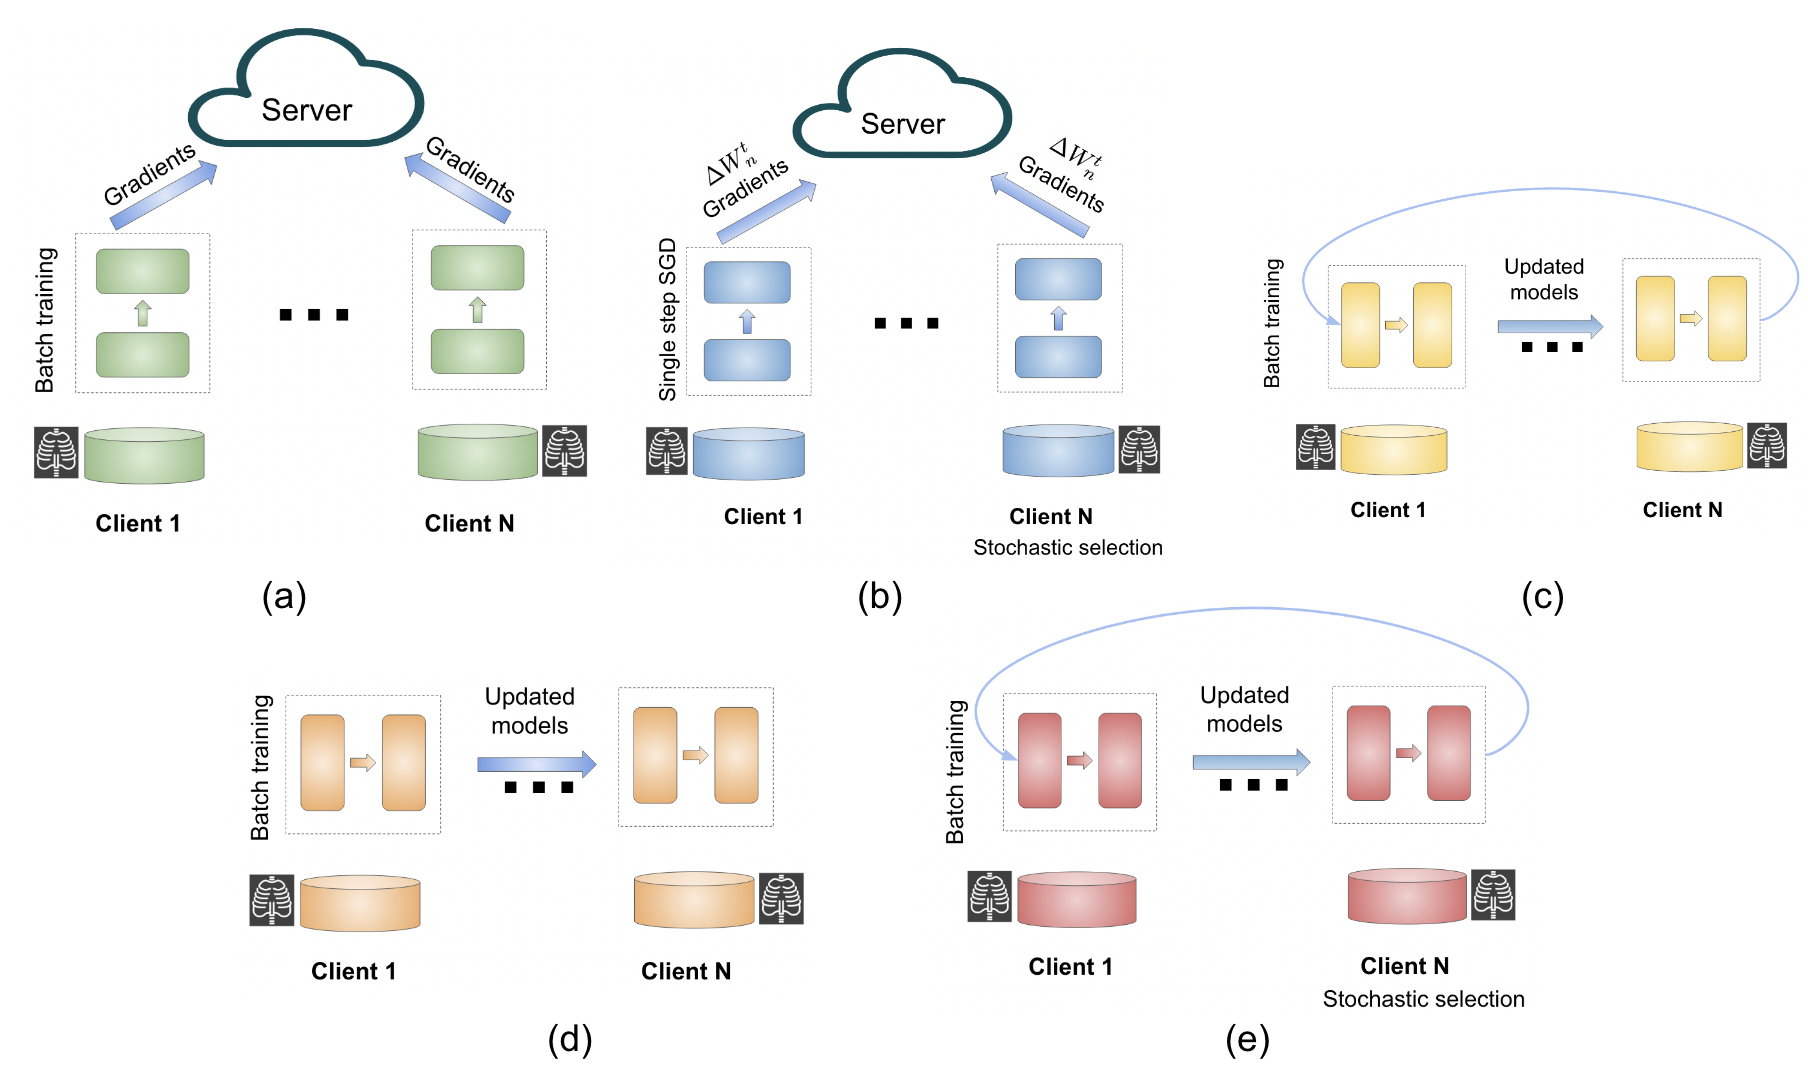
\includegraphics[width=1\textwidth]{FLmodels.png}
\caption{Illustration of FL models and algorithms: (a) Federated averaging, where clients train on a local batch of data. (b) FedSGD, in which a subset of clients is selected, and each performs a single step of SGD before sending model updates to the server. (c) Cyclic Weight Transfer (CWT), where clients train locally and pass the model to the next client, repeating the cycle. (d) Single Weight Transfer (SWT), where the model passes through each client only once. (e) Stochastic Weight Transfer (STWT), in which the model is sequentially passed through clients, with participating clients in each round being sampled randomly.}
\label{fig:flalgorithms}
\end{figure*}


Recent research has focused on the classification of scan images to distinguish between COVID-19 patients and healthy individuals, as well as identifying lesion areas. The primary application of AI in managing COVID-19 patients has been the interpretation of radiology images, especially chest CT scans.  The detection of lung alterations through these scans plays an important role in optimizing patient management and guiding treatment decisions\cite{yan2020interpretable}\cite{hu2020challenges}\cite{burian2020intensive}.  Several studies have also explored 3D Convolutional neural networks \cite{wang2020weakly} and COVID-19 detection with a limited number of training samples.

While the majority of these studies report favorable accuracy, they often presume a centralized environment wherein a single data center has access to all data. However, a few studies have successfully applied distributed learning for COVID-19 detection, employing global aggregation models such as model averaging in federated learning settings\cite{ho2022fedsgdcovid}\cite{zhang2021dynamic}, or within a blockchain framework \cite{kumar2021blockchain}. These studies have pointed to certain limitations of existing algorithms, such as high communication overhead \cite{remedios2020federated}, as well as convergence issues or catastrophic forgetting when the number of participating hospitals increases \cite{sheller2020federated} \cite{chang2018distributed}.


To our knowledge, no study has been performed that compared multiple FL algorithms under standard conditions to evaluate their applicability. Therefore, comparing multiple FL algorithms under standard conditions could be informative in evaluating their applicability in practice.

To evaluate the existing methods from multiple perspectives, we have implemented the most popular models and compared them in terms of performance, communication overhead, and computation burden.


\section{Algorithms}
% \label{sec:algorithms}
\textbf{Centralized Data Sharing} In Centralized Data Sharing (CDS), data is stored in a central location and is accessible to all clients. This stands in contrast to federated and decentralized data sharing methods, where data is stored across multiple locations and accessed by either a single user or a limited number of users. CDS serves as a baseline for comparing other algorithms.
\textbf{Federated Averaging} Federated Averaging involves an iterative learning procedure comprising local and global steps. In this process, each data owner trains a model received from a global server on its local dataset through local iterations \cite{mcmahan2017communication}. Subsequently, the global server aggregates the updated local models to update the global model. This global model is then distributed to clients for the subsequent round. The optimization problem for Federated Averaging can be expressed as:
\begin{equation}
w^{t+1} = \sum\limits_{i=1}^{N}{p_{i} w_{i}^{t}} , w_{i}^{t}=\arg\min\limits_{w_{i}}{\left(\mathcal{L}(\mathcal{D}_{i};w^{t})\right)}
\end{equation}
where $N$ is the number of data owners, $\mathcal{L}(\mathcal{D}_{i};w^{t})$ is a loss function indicating global model parameters  $w^{t}$ of local datasets, and $p_{i}$ is the probability of selecting client $i$. 
Local optimization can be formulated as $w_{i}^{t+1} \leftarrow w^{t}-\eta\cdot \nabla \mathcal{L}(w^{t};\mathcal{D}_{i})$, where 
 $\eta$ is the learning rate. The global model can be updated based on the local models $w_{i}$ and is shared for aggregation: 
\begin{equation}
w^{t+1} = \sum\limits_{i=1}^{N}{p_{i} w_{i}^{t+1}}
\end{equation}

\textbf{Federated Stochastic Gradient Descent} Federated Stochastic Gradient Descent, or FedSGD\cite{chai2020fedeval}, is a variant of Federated Averaging (FedAvg) that employs a large-batch synchronous approach for multi-client learning. In FedSGD, a subset of clients is chosen from the total pool, with this subset being defined by $C$. This selection is made at each global round. Subsequently, the global server dispatches the latest global model to the chosen clients. Each of these clients then undertakes local training on its dataset for a predetermined number of epochs. The global model is updated in light of the local models obtained from each client and is made available for aggregation, a process that is analogous to that in FedAvg. Nevertheless, FedSGD distinguishes itself by computing the gradient over the chosen batch of clients, hence $C < 1$. When $C = 1$, the training becomes non-stochastic, or full batch, as it involves all the clients. This makes it possible to train with large batches since the gradient is computed over the selected subset of clients.

The optimization problem for FedSGD can be expressed as follows:
\begin{equation}
w^{t+1} = w^{t} - \eta \cdot \sum\limits_{i=1}^{C}p_i \cdot \nabla \mathcal{L} (w^t;\mathcal{D}_i)
\end{equation}
where $\eta$ is the learning rate, $p_i$ is the probability of selecting client $i$ and $\mathcal{L}$ is the loss function.
The key difference between FedAvg and FedSGD lies in the use of large-batch synchronous approach in FedSGD. This approach has been shown to outperform the naive asynchronous SGD training due to the increased accuracy and efficiency, as compared to the local training approach used in FedAvg \cite{chai2020fedeval}\cite{charles2021large}. Additionally, FedSGD has been shown to be more robust to non-IID data distributions, compared to FedAvg \cite{chai2020fedeval}. 
\quickthings{This part is unclear to me.}
% \absolutelynecessary{}
\maybelater{paraphrised}

\textbf{Cyclic weight transfer} Federated learning techniques have been widely used in medical image processing tasks using a method known as cyclic weight transfer (CWT)\cite{balachandar2020accounting}. This method involves training models on individual clients for a number of iterations and then cyclically sharing the updated weights with the following client. However, the existing CWT algorithm faces a notable challenge, as it lacks the ability to effectively manage inter-client variability in training data or labels.  To ensure the practical application of CWT, it is crucial to develop a version that can handle the common variations observed in a majority of real-world medical imaging datasets\cite{darzidehkalanifederatedII}.

\textbf{Single weight transfer} Single weight transfer (SWT) is anothe FL method widely used in the medical imaging domain. In Single weight transfer, models are trained in each client with its local data, and then the updated model is transferred to the next client. The difference between this method and CWT is that here the model passes each client only once\cite{darzidehkalanifederatedI}. 

\textbf{Stochastic weight transfer}
In stochastic weight transfer (STWT), we select a subsample of clients and train them in a cyclic manner. Similar to FedSGD, a ratio defines the number of selected clients to the total number of clients in each federated round. 

Figure \ref{fig:flalgorithms} provides a visual representation of the introduced algorithms.



% سوال / مسیله چیه
% Importance: Why your research matters in the context of an industry or the world
% اهمیت موضوع
% 	کجاها کاربرد داره
% مشکلات موضوعات قبلی و اینکه مسایل دگ کار نمیکنن
% برای اینکه این مسایل کار کنن نیازی به چه چیزی بود. ک اونا کم داشتن
% چرا این روش تو داره کار میکنه
% چه سوالی رو جواب میده
% توضیح اینکه چجوری کار میکنه
% تعریف و تمجید از کار کردنش

% \maybelater{chanta akse tamiz ba coreldraw bekesh}

% Their
% We are comparing various implementations of FL and comparing their performance level. The performance is done by metrics.
% 2. Although FL has been introduced to tackle the problem of privacy, its distributed nature requires too much commuincation between clients. Knowsing can determine its deployability and scailibitlty. Hence the question is how to these model compare it terms of communication between clients.
% 3. Computation time. Each FL model is investigated based on the required time for computation.
% 4. Effect of rounds: Number of Federated rounds 


% \quickthings{Maybe you can add a benchmarking section similar to "A Performance Evaluation of FL Algorithms"}
% \maybelater{Some ideas are herer https://arxiv.org/pdf/1709.05929.pdf
% }





 
\section{Experiment}
\textbf{Dataset} Our experiments used two publicly available data sources, the Tongji hospital dataset\cite{yang2020covid} and Brazil's SARS-CoV-2 dataset\cite{soares2020sars} Tongji dataset consists of 349 chest CT-scans of COVID-19 positive and 397 scans of healthy subjects, all low-resolution CT modalities. Brazil's SARS-CoV-2 dataset consists of 2482 samples, 1252 scans of COVID-19-infected patients, and 1230 healthy subjects collected from multiple hospitals in Sao Paulo, Brazil. The datasets are approved by the corresponding ethical committees of each hospital, Public Hospital of Sao Paulo (HSPM), and Tongji Hospital in Wuhan, China. Train and test sets were obtained randomly from the aggregated datasets. Table \ref{table_datadist}, shows data distribution.


\begin{table}[h!]
\centering
\setlength{\tabcolsep}{6pt}
\renewcommand\arraystretch{1.22}
\caption{ \small Data distribution}
\begin{tabular}{| *{5}{c|} }
\hline
Class  & Dataset & Samples & Train & Test
\\   \hline  
\multirow{2}{3em}{COVID}     &Brazil&1252&\multirow{2}{2em}{1451}  &\multirow{2}{2em}{150}  \\
&Tongji&349&&  \\
\hline
\multirow{2}{6em}{Non-COVID}     &Brazil&1230&\multirow{2}{2em}{1477}  &\multirow{2}{2em}{150}  \\
&Tongji&397&&  \\
\hline
\end{tabular}
\label{table_datadist} 
\end{table}


\textbf{Preprocessing}
Images were selected as 2D slices in greyscale. Preprocessing included randomly cropping between 0.5 to full size, random horizontal flipping, and intensity normalization. CT-slices were all resized to 224$\times$224 pixels with interpolation. Figure \ref{fig:samplesCTs} shows samples of processed images.
% \quickthings{This looks like you have a bias in your dataset. You should select the normals and abnormals at comparable level in the thorax. All covid are now lower in the body then the non-covid ones.}
% \maybelater{I have changed the picture, hope it's okay now}
\begin{figure}[h!]
 \centering
 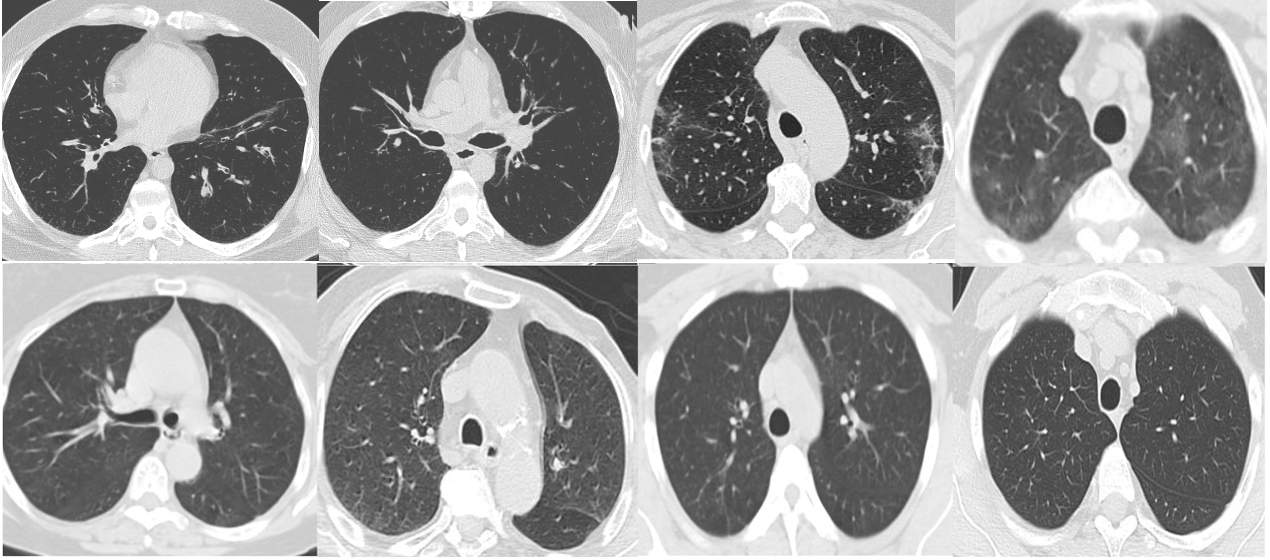
\includegraphics[width=0.45\textwidth]{covidexamples3.png}
 \caption{Sample CT slices of COVID-19 images (top row) and Non-COVID images (bottom row)}
 \label{fig:samplesCTs}
\end{figure}


% normalize = transforms.Normalize(mean=[0,0,0], std=[1,1,1])
% train_transformer = transforms.Compose([
%     transforms.Resize(256),
%     transforms.RandomResizedCrop(224, scale=(0.5, 1.0)),
%     transforms.RandomHorizontalFlip(),
%     transforms.ToTensor(),
%     normalize
% ])

\textbf{Training}
ResNet-18 is used as the backbone deep learning model. ResNet-18 comprises one initial block cascaded to four middle blocks. The initial block is made of convolutional,  batch normalization, ReLU, and pooling layers. Middle blocks have the same layers, connected with straight and skip connections. The model is pre-trained on ImageNet dataset \cite{he2016deep} with a CrossEntropy loss function and learning rate of $0.05$. 
Each federated round consisted of 20 internal epochs for each client and batches of 16 samples in each iteration. For models which use minibatch training, like STWT and FedSGD, a subset of clients is randomly selected. Similar to training, test data was split into mini-batches, and the results were averaged across batches. We performed training with various participating clients and federated rounds to evaluate their effect on final performance. Models were also trained in a centralized, non-federated setting to build a comparison baseline. Figure \ref{fig:distributionsite} shows the data distribution among clients.

\begin{figure}[h!]
 \centering
 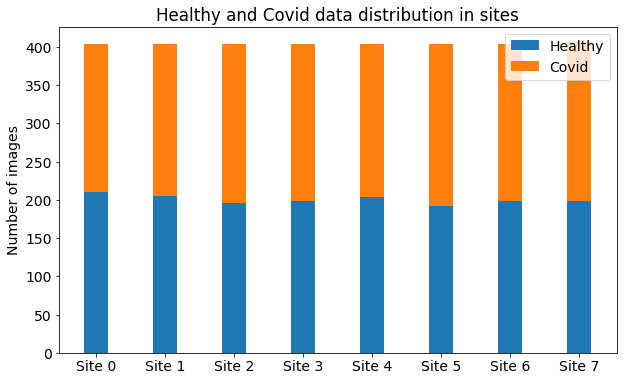
\includegraphics[width=0.7\textwidth]{output.png}
 \caption{Data distribution of each client in the simulated federated setting}
 \label{fig:distributionsite}
\end{figure}
% \abs{Healthy COVID data distirbution per site}

\textbf{Evaluation} 
Standard classification metrics, accuracy, recall, precision, and F1 score, were used as our evaluation criteria. We also evaluated the level of communication, the amount of transferred data in each algorithm, and the computational complexity of the models. 
\label{sec:experiment}


\section{Results}


% In order to evaluate and compare federated learnign models 
% Specificity  and  sensitivity  are  the  abilities  of  a  model  that how correctly the model identifies a subject with disease and without a disease. 
% In our case, it is critical to detect a COVID-19 patient as missing a COVID-19 patient can have disastrous consequences.   

% A medical diagnosis based system needs to have high sensitiv- ity and recall. 
Here, the result for the setting with 10 participating clients and a maximum of 10 rounds is presented. The results are average performance among clients for all the federated rounds. Table \ref{best_performance} shows the results.
% \quickthings{Why comparison of FedAVG and CWT?}\maybelater{I removed the sentence}
% The average score in each state could be a way to reach them—the average scores in F1, FedSGD, CWT, and SWT. 
% The FedSGD models have been used are
% The results for CDS are also included as a benchmark ground truth.

% \quickthings{Put CDS at the top, keep same order as in the materials and methods. Consistency!}
% \maybelater{Fixed!}

\begin{table}[h!]
\centering
\setlength{\tabcolsep}{5.5pt}
\renewcommand\arraystretch{1.12}
\caption{ \small Comparison of FL algorithms on classification of COVID-19 data for 10 clients, averaged performance in all the 10 rounds.}
\begin{tabular}{| *{5}{c|} }
\hline
Method & Accuracy & Recall & Precision & F1 score
\\
  \hline
  

CDS
 &87.75\%&89.57\% &87.93\% & 87.19\%  
\\   \hline  
FedAVG
 & 66.72\% &70.02\% &43.80\% & 51.7\%\\ 
 \hline  
FedSGD
 &65.17\% &68.24\%&43.86\%& 47.75\%  
 
 \\
 \hline  
CWT
 &87.75\%&89.00\%& 88.67\%&87.52\%\\
 
   \hline
 

SWT
 & 64.60\% &74.33\% & 65.55\% &59.66\% \\
    
\hline 
STWT
 & 84.21\% &84.09\%&83.33\% & 81.71\%  \\



\hline
\end{tabular}
\label{best_performance} 
\end{table}


\textbf{Assesing the impact of training rounds} To evaluate the effect of number of rounds, models with 3, 5, 10 and 15 rounds were tested. The test results are shown for both centralized and FL  algorithms. Table \ref{number_of_rounds} shows the results of our experiment. The increasing number of rounds correlates with higher accuracy of the global model.
% \quickthings{Same with table III, put at the top.}

% \maybelater{done}

% \begin{table}[h!]
% \centering
% \setlength{\tabcolsep}{5.5pt}
% \renewcommand\arraystretch{1.12}
% \caption{ \small Effect number of rounds on models' accuracy}
% \begin{tabular}{| *{5}{c|} }
% \hline
% Method & 3 rounds & 5 rounds & 10 rounds & 15 rounds 
% \\   \hline  
% FedAVG
%  & 66.28\% &77.24\% & 86.63\% & 94.03\%\\

%  \hline
%  FedSGD
%  &  53.77\% & 70.55\% &90.04\% & 92.75\%\\
% \hline  
% % SWT
% %  &  85.34\% & 97.24\% &93.63\% & 98.74\%\\
% % \hline  
% CWT
%  &  96.02\% & \textbf{98.44\%} &\textbf{99.29\%} & 99.86\%\\

% % \hline  
% % CDS
% %  to be completed!


% \hline  
% STWT
%  &  \textbf{96.59\%} & 97.72\% &99.57\% & \textbf{100.00\%}\\

 
%  \hline
% CDS
%  &92.03\% &88.34\% & 98.01\% & 100.00\% \\
%  \hline
% \end{tabular}
% \label{number_of_rounds} 
% \end{table}


\begin{table}[h!]
\centering
\setlength{\tabcolsep}{3.5pt}
\renewcommand\arraystretch{1.12}
\caption{ \small Effect number of rounds on accuracy of FL algorithms for 10 clients, 20 internal epochs.}
\begin{tabular}{| *{5}{c|} }

% \begin{tabular}{| {c|}{c|}{c|}{c|}{c|}{c|}{c|}{c|}{c|} |}
\hline
% Method & \multicolumn{2}{c}{3 rounds} & \multicolumn{2}{c}{5 rounds} &\multicolumn{2}{c}{10 rounds} &\multicolumn{2}{c}{15 rounds} 

Method & 3 rounds & 5 rounds & 10 rounds & 15 rounds
%  & M &SD & M &SD& M &SD& M &SD 
\\
 \hline
CDS
 &85.06\% &81.56\% & 91.06\% & 91.04\% 
\\
\hline
FedAVG
 & 56.05\%  &63.78\%&69.64\%&70.73\% \\

 \hline
 FedSGD
 &  50.88\% & 55.9\% &75.59\% & 76.94\%\\
% \hline  
% SWT
%  &  85.34\% & 97.24\% &93.63\% & 98.74\%\\
\hline  
CWT
 &  80.77\% & \textbf{89.78\%} &\textbf{91.27\%}& \textbf{93.56\%}\\

% \hline  
% CDS
%  to be comp,';leted!


\hline  
STWT
 &  \textbf{90.73\%} & 83.97\% &89.44\% & 93.01\%\\

 
  \hline

\end{tabular}
\label{number_of_rounds} 
\end{table}
\quickthings{Shouldn't this column have the same results as table II for accuracy?}

\peter{Table III and Table II do not represent the same thing. Table II is average performance in all 10 rounds, is to give an overall impression of accuracy, and table III is the final result in the end of the 5th, 10th , 15th rounds.  Added  to the table caption.
}
% \maybelater{The results are for max, maybe you want to add average results later?}
% \maybelater{Having the same thing (acc) for other metrics such as F1, prevciison recall etc}

\textbf{Assessing the influence of client participation}
To evaluate the number of clients on the FL network, we examined scenarios with 3,5, and 8 participating clients. We trained each of the clients in 20 internal epochs. The number of Federated rounds for all the algorithms (except SWT) was 10.
The average test results are shown in the Figure \ref{fig:data distribution}. \quickthings{Why not a column for 10 clients here?}
\maybelater{ 10 clients are shown in table three , third column. Added 10 clients here as well}

% \begin{table}[h!]
% \centering
% \setlength{\tabcolsep}{7pt}
% \renewcommand\arraystretch{1.22}
% \caption{ \small Effect number of clients on accuracy of FL algorithms, 10 rounds, 20 internal epochs.}
% \begin{tabular}{| *{9}{c|} }
% \hline
% Method & 3 clients & 5 clients & 8 clients 
% \\   \hline  
% FedAVG
%  & 79.52\% &70.73\% & 63.98\% \\

% \hline  
% FedSGD
%  & 78.02\% &75.59\% &69.76\%  \\
% \hline  
% CWT
%  &  89.90\% & \textbf{91.27\%} &\textbf{88.98\%} \\
%  \hline
% STWT
%  &  \textbf{90.93\%} & 89.44\% &84.57\% \\
%  \hline  
% SWT
%  & 55.80\% &69.19\% & 68.81\%\\




% \hline  
% CDS
%  to be completed!

% \hline  

% \end{tabular}
% \label{effect_num_clients} 
% \end{table}


\begin{figure}[h!]
 \centering
 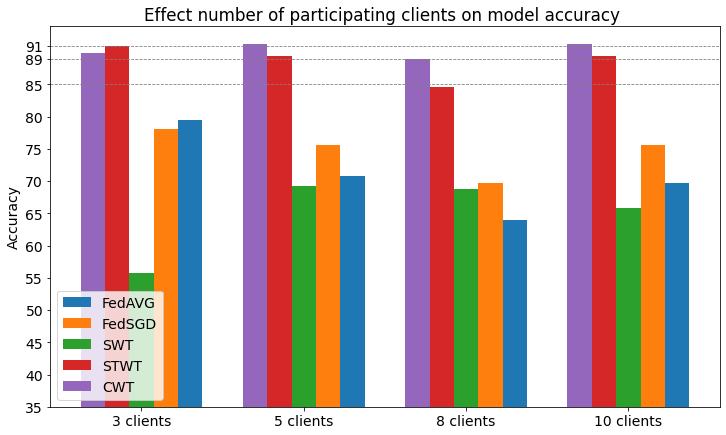
\includegraphics[width=0.7\textwidth]{download.png}
 \caption{Accuracy of FL algorithms with differrent number of clients. }
 \label{fig:data distribution}
\end{figure}


% \maybelater{Maybe taking MAX is better instead of latest epoch?}

 
\begin{figure}[h!]
 \centering
 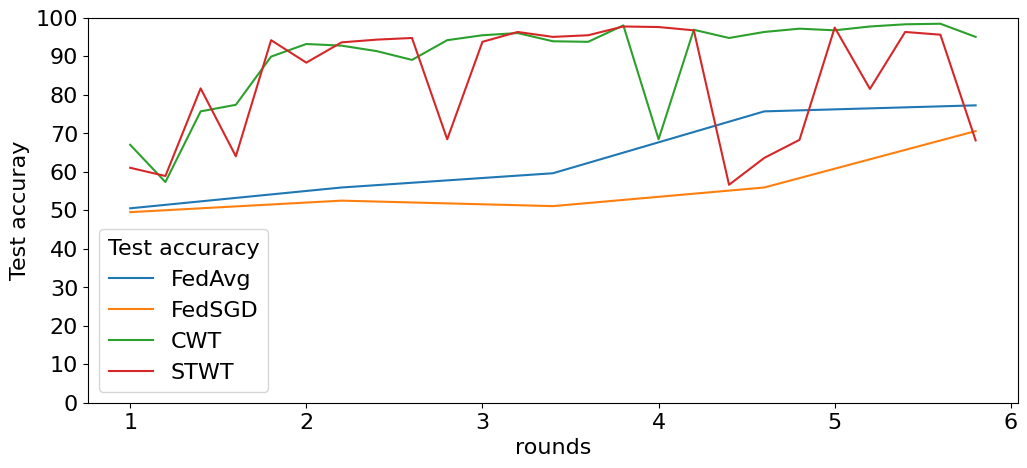
\includegraphics[width=0.7\textwidth]{cyclic.png}
 \caption{Test accuracy as a function of passing rounds}
 \label{seq-vs-noseq}
\end{figure}
% \maybelater{Best accuracy vs Average accuracy for showing that SWTW works bad in average but well in best accuracy}
% \abs{Adding a graph showing arrows for gradient updates}
% \maybelater{Maybe adding 10 clients?}
% \maybelater{8 ta client, 4 FL rounds
% 20 each client for CWT plot . and also 8 ta client, 4 FL round 20 each client for FedSGD and FedAVG}
% \subsection{Other graphs}

\begin{table}[h!]
\label{computation time}
\centering
\setlength{\tabcolsep}{7pt}
\renewcommand\arraystretch{1.22}
\caption{ \small Computation time (seconds) for FL algorithms for standardized setting}
\begin{tabular}{| *{9}{c|} }
\hline
Method & 3 clients & 5 clients & 8 clients  & 10 clients
\\   \hline  
FedAVG
 & 8934 sec&8975 sec  & 9002 sec & 9030 sec\\

\hline  
FedSGD
 & 8810 sec &8853 sec& 9013 sec & 9052 sec \\
\hline  
CWT
 &  5119 sec& 5450 sec&5383 sec & 5556 sec\\
 \hline
STWT &
2805 sec&  5243 sec& 6101 sec & 6129 sec\\
 \hline  
SWT
 & \textbf{543 sec} &\textbf{547 sec} & \textbf{589 sec } & \textbf{618 sec}\\



% \hline  
% CDS
%  to be completed!

\hline  

\end{tabular}
\label{computation_time} 
\end{table}


Communication can also be a bottleneck in this setting. In methods like federated averaging, the lower bounds for total communicated data are proportional to $\sim$
${2NT}$
where the total rounds are represented by T and the count of involved clients is denoted by N. In CWT, this lower bound is  $\sim$ ${NT}$. In our setting, we use a ResNet 101 model. We calculated the overall transferred data for the different number of rounds. As expected, the experiments show that when clients are selected randomly, the communication time tends to be shorter compared to scenarios involving participation from all clients. Moreover, our analysis of computational costs indicates that models that do not rely on sequential processing generally demand higher computational resources compared to their sequential counterparts. The detailed results for computational and communication evaluations can be found in Table \ref{computation_time} and Table \ref{transferredData}, respectively.
\quickthings{Again, why only this comparison is relevant enough to put into the text?}
\maybelater{Here fedavg, and fedsgd are the same family, (non sequential), and CWT are the other family (sequential)., Changed the phrasing from CWT/FedAVG to seq/non-seq, hope it's okay this time.}

\begin{table}[h!]
\centering
\label{Transferred data}
\setlength{\tabcolsep}{5.5pt}
\renewcommand\arraystretch{1.12}
\caption{ \small Comparison of total transferred data in a normalized setting (GB)}
\begin{tabular}{| *{5}{c|} }
\hline
Method & 3 rounds & 5 rounds & 10 rounds & 15 rounds 
\\   \hline  
FedAVG
 & 1.371 &2.286 & 4.571 & 6.857\\

 \hline
 FedSGD
 &  0.823 & 1.371 &2.743 & 4.114\\
\hline  
% SWT
%  &  85.34\% & 97.24\% &93.63\% & 98.74\%\\
% \hline  
CWT
 &  0.686 & 1.143 &2.286 & 3.428\\

% \hline  
% CDS
%  to be completed!


\hline  
STWT &
  0.411 & 0.686 &1.371 & 2.057\\

 

 \hline
\end{tabular}
\label{transferredData} 
\end{table}





% \maybelater{Momkene computational complexity ro beshe ba order nevesht? peida kon settingesh ro}
% \maybelater{Graphs showing results}
% \maybelater{Comparison of FL models}
% \maybelater{Loss/round}
% \abs{definition of precision and recall}


\label{sec:results}



% \newpage


\section{Discussion}
\label{sec:discussion}

% Local training had near random accuracy, but in all the experiments, the performance results were improved. 
% Considering low number of samples for individual clients, a training process limited to few clients results in near random classification accuracy. 
% Local models can have low performance due to limited datasets.
% Also,, ImageNet pre-training had a speed-up effect on our model performance.

% \textbf{Fundamental groups of FL}

% \textbf{how many groups}
% \textbf{how can we group them, name different ways}
% \textbf{effect number of data}


% Paragraph 1: This paragraph provides a “big picture” perspective for readers to remind them of the importance of your study.

% \textbf{overall results}
% 
Our results show that FL has comparable performance to centralized data sharing, with the advantage of keeping data private. With large volumes of data and after high number of rounds, centralized data sharing and cyclic weight transfer have the highest accuracy. 


Sequential models are susceptible to catastrophic forgetting, where a global model performs well on the latest client it has seen while having poor performance in other clients.\quickthings{cryptic sentence}\maybelater{I have paraphrised the sentence}
Conversely, in algorithms like FedAvg and FedSGD, the models are averaged asynchronously after all the clients have finished their training. So the trajectory is smoother and overall improving with more communication rounds. As shown in Figure \ref{seq-vs-noseq}, local test results can have a high variance when passing through clients sequentially, indicating the catastrophic forgetting effect.

Models like FedAvg, and FedSGD, in which all the clients have identical copies of one global model, are slower and more challenging to converge compared to sequential models like CWT and STWT. Also, FedAvG and FedSGD require more training resources due to active server participation, resulting in more computation and network consumption. Stochastic client selection is an efficient way of training. Stochastic models save significant time and resources while having similar performance to full client participation. Overall, CWT and STWT have best results in terms of model accuracy and computation times. These findings could be practical in further federated deployments in medical institutions.
% but when there are communication and computation limitations, other methods might be more practical.




% As can be seen in the results, CWT and STWT have better local results than other methods.

% So each local model is different than other models, and even in fewer rounds they retrain the model on their local data and achieve high accuracies. 

%  Unsurprisingly, CDS has higher accuracy than non-sequential methods.
 
% so in limited number of rounds, latter algorithms are preferred.



%  FedAVG needs to perform both local training and global aggregation, which requires is to have more computation, than sequential models which eliminate global aggregation and broadcasting step.   
%  Models with global server, suh as FedAVG and FedSGD, required more data transfer, because of the two way communication of each client with server.
Sequential models like CWT and STWT perform better than non-sequential models on fewer training rounds. For example,  after three rounds of training, STWT and CWT both reach 96\% accuracy, while FedAvG reaches 66\%, and FedSGD performs equally to a random classifier. As the training proceeds, FedAVG and FedSGD gradually improve with more global rounds.The concept of sequential models is similar to fine-tuning \cite{chen2020online} in centralized deep learning, so in cases where a hospital temporarily joins an FL network, or there is an urgency in training, sequential models are a better option.

More training rounds do not always lead to a better global model. Although average performance on all clients improves, more global rounds lead to worse performance for some clients. The global model can overfit some clients, leading to lower performance on others\cite{mohri2019agnostic}. Some studies suggested early stopping and fine-tuning to local dataset after global training is finished \cite{yu2020salvaging}. 
In all the algorithms, more clients resulted in slower convergence. This effect is stronger in the FedAvg algorithm. In FedAVG, the Global model must compromise between potentially disparate local minima\cite{li2019convergence}. Methods such as adaptive or stochastic selection of clients and momentum-based models help faster convergence \cite{liu2020accelerating}.
Our results suggest that stochastic client participation is close to full client participation. The average results of four trials with varying rounds, shown in Table \ref{number_of_rounds} indicate that stochastic client participation in FedSGD results in 5.23\% performance loss and 40\% less bandwidth consumption compared to FedAvg. In STWT, it results in only 1.25\% less accuracy but saves 40\% of communication and 11.3\% of computation.
% Also, SWT improves local clients' performance up to 80\% accuracy with 8 clients, and it requires extremely low bandwidth requirements.
These results are in accordance with prior studies, showing that, in theory, stochastic and full client participation have similar global minima\cite{cho2020client}. Stochastic client selection can be advantageous when there are limited resources, or in larger networks with occasionally unavailable clients.


% Models like FedSgd and STWT, select the participating clients in a stochastic manner. 
% The reason is because each client has less data, and there will be more number distant local client minima leading to unstable global model.


% Such can be a reflection of real world setting, where not all the clients are active in each round. So a fraction are selected.


% Some models have high max test accuracy while average is low indicating bias and catastrophic forgetting. Infrastructure limitations should be considered, when a central server has limited computing power it would be unable to perform FedAVG, instead no-server algorithms require to pass the model to the next client.

We did not assume any shift in clients' data. A more comprehensive analysis should consider the effect of the domain and distribution shifts on the performance of the algorithms. Also, inter-client data variability and the effect of heterogenous clients could be a future line of research.
% For deployments in longer timeframes, there might be changes in clients data distirbution , and previous results might be inapplicable Effect of domain shifts, and inter-client data variability could be a future line of research. 






\section{Conclusion}
\label{sec:conclusion}
 
FL enables extensive collaborations of hospitals to address medical imaging problems while keeping data private. Real-world implementation requires consideration of efficiency and hardware requirements in addition to model performance, especially in the healthcare field, which generally has limited infrastructure. We implemented five FL algorithms for COVID-19 detection and analyzed their efficiency and accuracy.
Our results suggest that FL algorithms have comparable performance to centralized data sharing, with the advantage of keeping data private. They also show that the sequential methods are a better option in most of the scenarios. This study can be helpful in the deployment of FL systems in COVID-19 detection and medical image analysis in general.

% demonstrate better performance for detecting COVID-19 patients and might be practical in deploying FL algorithms for covid-19 detection and medical image analysis in general.





\printbibliography






% \section*{Acknowledgement}



\ifCLASSOPTIONcaptionsoff
  \newpage
\fi



\bibliographystyle{IEEEtran}
\bibliography{IEEEabrv}



\vfill
% \section{To do list}
% \subsection{Quick things}

% \subsection{Absolutely necessary}

% %   \item add pathology image to figure perturbation of MRI
% \subsubsection{Paper}
% \begin{itemize}
%     % \item paraphrise + shorten FL and DP sections
%     % \item baad yebar ba dide Chaoning bekhun
% \end{itemize}
% \subsubsection{Coding}
% \begin{itemize}

% \end{itemize}
% \subsection{Maybe later}
% \subsubsection{coding}
% \maybelater{CWT but with random ordering}
% \maybelater{One shot FL?}
% \maybelater{Vazne kamtari dadan be latest client in CWT ?}
% \maybelater{Testing with other deep networks?}
% \maybelater{At least you can increase depth of network}
% \maybelater{Impact of data heterogeneity? just split the data heterogeneously and see how do they work?}

% \maybelater{Effect of Differential privacy?}
% \maybelater{Effect of pretrained=False?}
% \maybelater{HasSpike model?}
% \maybelater{Maybe small variations to generate new models}
% \maybelater{Maybe doing gradient masked FedAvG?}
% \maybelater{Maybe evaluating different number of local epochs like https://github.com/siddarth-c/FedGMA}
% \maybelater{Adding all these ideas to Obsidian/presentations}
% \maybelater{Going for another paper if an idea is worth pursuing}
% \maybelater{Another paper: CWT/SWT with DP}
% \maybelater{Local GD like Ahmed khaled}

% \subsubsection{Paper}
% \begin{itemize}
%     \maybelater{Adding mathematical expression of each FL model (good to improve math level of paper)}
%     \maybelater{maybe adding detailed graph for each participant as an Appendix?}
%     \maybelater{Adding algorithmic view of each FL alg?}
  
% \end{itemize}





% that's all folks
\end{document}



\include{watchdog-tse/paper}
\include{travis-analysis/structure}
\include{debugging/paper}
\chapter{Conclusion}
\label{conclusion}

The conclusions of your thesis.

\chapter*{Acknowledgements}
\addcontentsline{toc}{chapter}{Acknowledgements}
\label{acknowledgements}

This is an optional chapter containing acknowledgements.


%% Use letters for the chapter numbers of the appendices.
%\appendix

%\include{appendix-a/appendix-a}

%% Turn off thumb indices for unnumbered chapters.
\thumbfalse

\chapter*{Bibliography}
\addcontentsline{toc}{chapter}{Bibliography}
\setheader{Bibliography}

URLs in this thesis have been archived on Archive.org. Their link target in digital editions refers
to this timestamped version.

% argument is your BibTeX string definitions and bibliography database(s)
\bibliographystyle{unsrt}
\bibliography{dissertation,./asats/paper,./last-line/bib,./watchdog-tse/paper,./travis-analysis/structure,./debugging/paper}

\chapter*{Curriculum Vit\ae}
\addcontentsline{toc}{chapter}{Curriculum Vit\ae}
\setheader{Curriculum Vit\ae}

%% Print the full name of the author.
\makeatletter
\authors{\@firstname\ {\titleshape\@lastname}}
\makeatother

\noindent
\begin{longtable}{p{.225\textwidth} p{.70\textwidth}}
     & Date of birth in Tehran, Iran.
\end{longtable}



\chapter*{List of Publications}
\addcontentsline{toc}{chapter}{List of Publications}
\setheader{List of Publications}
\label{publications}

%% We use the 'etaremune' environment (the reverse of 'enumerate') to get a
%% numbered list of publications in reverse chronological order. If the list of
%% authors is long, it might be useful to emphasize your own name with \textbf.
\begin{etaremune}{\small
\item[\faFileTextO~~1.] \emph{Moritz Beller}: Toward an Empirical Theory of
  Feedback-Driven Development. To appear in 40th International Conference on
  Software Engineering (ICSE), Student Research Competition (SRC),
  Gothenborg, Sweden, 2018. Acceptance Rate 43\% (10/23)
}\end{etaremune}

\vspace{0.5cm}
\noindent
\faFileTextO~~Included in this thesis.\\
\faTrophy~~Won a best paper, tool demonstration, or proposal award.


\end{document}

